% !TEX program = xelatex
% ============================================================================
% មគ្គុទ្ទេសក៍គរុកោសល្យគ្រូ និងរបាយការណ៍ស្រាវជ្រាវ (Teacher's Guideline -- RN1)
% មុខវិជ្ជា៖ គណិតវិទ្យា ថ្នាក់ទី៨ (ផ្នែកពីជគណិត) -- មេរៀនទី១៖ ចំនួនសនិទាន
% ចំណុចរង៖ ១. សញ្ញាណចំនួនសនិទាន (ទំ.១--២ & ១១: #1, #3(ក,គ), #4(ក–ង))
% គ្រូបង្រៀន៖ ហុក ប៊ុនថែន | អនុវិទ្យាល័យព្រះក្រសាំង (កំពង់ស្វាយ-កំពង់ធំ)
% Mobile-First Readability Standard: 11.5pt / 18.2pt, top/bottom=2.30cm, breakable boxes
% ============================================================================
\documentclass[a4paper,12pt]{article}

\usepackage[a4paper, left=1.45cm, right=1.45cm, top=2.30cm, bottom=2.30cm, headheight=18pt, headsep=0.68cm, footskip=0.88cm]{geometry}
\usepackage{amsmath, amssymb}
\usepackage{unicode-math}
\usepackage{fontspec}
\usepackage{array, longtable, multirow, colortbl, booktabs}
\usepackage[table]{xcolor}
\usepackage{enumitem}
\usepackage{pifont}
\usepackage{fancyhdr}
\usepackage{lastpage}
\usepackage{needspace}
\usepackage[hyphens]{url}
\usepackage{tikz}
\usepackage[most]{tcolorbox}
\usetikzlibrary{calc, arrows.meta, positioning, babel}
\urlstyle{same}

% LaTeX 2025 + longtable v4.24 compatibility guard
\makeatletter
\let\@expl@@@mark@update@singlecol@structures@@\relax
\makeatother

% ============================================================================
% ការកំណត់ពុម្ពអក្សរផ្លូវការ (Cross-Platform Windows + Cloud fonts/)
% ============================================================================
\providecommand{\NGSFindFonts}{%
  \IfFileExists{C:/Windows/Fonts/cambria.ttc}{%
    \def\NGSSysPath{C:/Windows/Fonts/}%
    \def\NGSUserPath{C:/Users/KIT/AppData/Local/Microsoft/Windows/Fonts/}%
  }{%
    \IfFileExists{./fonts/KhmerOSsiemreap.ttf}{\def\NGSSysPath{./fonts/}\def\NGSUserPath{./fonts/}}{%
    \IfFileExists{../fonts/KhmerOSsiemreap.ttf}{\def\NGSSysPath{../fonts/}\def\NGSUserPath{../fonts/}}{%
    \IfFileExists{../../fonts/KhmerOSsiemreap.ttf}{\def\NGSSysPath{../../fonts/}\def\NGSUserPath{../../fonts/}}{%
    \IfFileExists{../../../fonts/KhmerOSsiemreap.ttf}{\def\NGSSysPath{../../../fonts/}\def\NGSUserPath{../../../fonts/}}{%
    \IfFileExists{../../../../fonts/KhmerOSsiemreap.ttf}{\def\NGSSysPath{../../../../fonts/}\def\NGSUserPath{../../../../fonts/}}{%
    \IfFileExists{../../../../../fonts/KhmerOSsiemreap.ttf}{\def\NGSSysPath{../../../../../fonts/}\def\NGSUserPath{../../../../../fonts/}}{%
    \IfFileExists{../../../../../../fonts/KhmerOSsiemreap.ttf}{\def\NGSSysPath{../../../../../../fonts/}\def\NGSUserPath{../../../../../../fonts/}}{%
      \def\NGSSysPath{../../../../../../../fonts/}\def\NGSUserPath{../../../../../../../fonts/}%
    }}}}}}}%
  }%
}
\NGSFindFonts

\setmathfont[
  Path={\NGSSysPath},
  FontIndex=1,
  Scale=1.06
]{cambria.ttc}

\defaultfontfeatures{Ligatures=TeX}

\setmainfont[
  Path={\NGSUserPath},
  Extension=.ttf,
  Script=Khmer,
  BoldFont={KhmerOSsiemreap},
  BoldFeatures={FakeBold=1.8},
  ItalicFont={KhmerOSsiemreap},
  ItalicFeatures={FakeSlant=0.25},
  BoldItalicFont={KhmerOSsiemreap},
  BoldItalicFeatures={FakeBold=1.8, FakeSlant=0.25}
]{KhmerOSsiemreap}

% ហាមដាក់ FakeBold លើ KhmerOSmuollight និងត្រូវរុំតួអក្សរឡាតាំង/លេខ ASCII ក្នុង \enbf{...}
\newfontfamily\muol[
  Path={\NGSUserPath},
  Extension=.ttf,
  Script=Khmer
]{KhmerOSmuollight}

\newfontfamily\TimesEn[
  Ligatures=TeX,
  Path={\NGSSysPath},
  Extension=.ttf,
  Scale=1.02,
  BoldFont={timesbd},
  ItalicFont={timesi},
  BoldItalicFont={timesbi}
]{times}

\newfontfamily\Tacteing[
  Path={\NGSUserPath}
]{TACTENG.TTF}

\newfontfamily\CourierBullet[
  Path={\NGSSysPath},
  Extension=.ttf
]{cour}

% ក្បួនកាត់ពាក្យខ្មែរ (Khmer word wrapping)
\XeTeXlinebreaklocale "km"
\XeTeXlinebreakskip = 0pt plus 1pt minus 0.1pt

% Mobile-First comfortable line spacing (11.5pt / ~18.2pt effective)
\linespread{1.22}

% ============================================================================
% ពណ៌ ស-ខ្មៅ (Strict Monochrome Palette) & Header/Footer Clearance
% ============================================================================
\definecolor{headgray}{HTML}{F2F2F2}
\definecolor{panelgray}{gray}{0.94}
\definecolor{stepgray}{HTML}{D9D9D9}
\definecolor{midgray}{gray}{0.82}
\definecolor{bordergray}{gray}{0.45}

\pagestyle{fancy}
\fancyhf{}
\renewcommand{\headrulewidth}{0.4pt}
\renewcommand{\footrulewidth}{0.4pt}
\fancyhead[L]{\rule[-3pt]{0pt}{14pt}\fontsize{9.5pt}{13pt}\selectfont មគ្គុទ្ទេសក៍គរុកោសល្យគ្រូ \en{(Grade 8 RN1)}}
\fancyhead[R]{\rule[-3pt]{0pt}{14pt}\fontsize{9.5pt}{13pt}\selectfont មេរៀនទី១ \en{(}១. សញ្ញាណចំនួនសនិទាន\en{)}}
\fancyfoot[L]{\rule{0pt}{13pt}\fontsize{9.5pt}{13.2pt}\selectfont កញ្ចប់ឯកសារ \en{NGS 5Es} \en{(}៥០ នាទី\en{)} \en{|} ហុក ប៊ុនថែន}
\fancyfoot[R]{\rule{0pt}{13pt}\fontsize{9.5pt}{13.2pt}\selectfont ទំព័រ \en{\thepage\ / \pageref{LastPage}}}

\fancypagestyle{firstpage}{%
  \fancyhf{}%
  \renewcommand{\headrulewidth}{0pt}%
  \renewcommand{\footrulewidth}{0.4pt}%
  \fancyfoot[L]{\rule{0pt}{13pt}\fontsize{9.5pt}{13.2pt}\selectfont កញ្ចប់ឯកសារ \en{NGS 5Es} \en{(}៥០ នាទី\en{)} \en{|} អនុវិទ្យាល័យព្រះក្រសាំង}%
  \fancyfoot[R]{\rule{0pt}{13pt}\fontsize{9.5pt}{13.2pt}\selectfont ទំព័រ \en{\thepage\ / \pageref{LastPage}}}%
}

\setlength{\parindent}{0pt}
\setlength{\parskip}{3.0pt}
\setlength{\tabcolsep}{4pt}
\setlength{\emergencystretch}{2em}
\setlist{itemsep=2.5pt, parsep=0pt}

% ============================================================================
% ម៉ាក្រូជំនួយ និងឋានានុក្រម \muol គ្មានតួអក្សរ ASCII បន្លំ (\Needspace <= 2.2cm)
% ============================================================================
\newcommand{\en}[1]{{\TimesEn #1}}
\newcommand{\enbf}[1]{{\TimesEn\textbf{#1}}}
\newcommand{\enit}[1]{{\TimesEn\textit{#1}}}
\newcommand{\unit}[1]{\,\text{\en{#1}}}
\newcommand{\cnum}[1]{\mbox{\TimesEn\fontsize{10.5pt}{12pt}\selectfont\ding{\numexpr181+#1\relax}}\hspace{0.15em}}
\newcommand{\ditem}{\tikz[baseline=-0.5ex]\fill (0,0.40ex) -- (0.40ex,0) -- (0,-0.40ex) -- (-0.40ex,0) -- cycle;\hspace{0.25em}}
\newcommand{\wcirc}{{\CourierBullet\fontsize{9.8pt}{11pt}\selectfont o}}
\newcommand{\chkbox}{\tikz[baseline=-0.15ex]\draw[black, line width=0.85pt] (0,0) rectangle (0.25cm,0.25cm);}
\newcommand{\khmflourish}{{\Tacteing\fontsize{38pt}{15pt}\selectfont\raisebox{-5pt}{3}}}

\newcommand{\parttitle}[1]{{\muol\fontsize{13.5pt}{17.5pt}\selectfont #1}}
\newcommand{\sectitle}[1]{{\muol\fontsize{12pt}{15.5pt}\selectfont #1}}
\newcommand{\subsectitle}[1]{{\muol\fontsize{11.5pt}{15pt}\selectfont #1}}
\newcommand{\tblhead}[1]{{\muol\fontsize{10.2pt}{15pt}\selectfont #1\par}}

\newcolumntype{L}[1]{>{\raggedright\arraybackslash}p{#1}}
\newcolumntype{C}[1]{>{\centering\arraybackslash}p{#1}}
\newcolumntype{R}[1]{>{\raggedleft\arraybackslash}p{#1}}

\newcommand{\secbanner}[2]{%
  \Needspace{2.2cm}%
  \vspace{2pt}%
  \begin{tcolorbox}[
    enhanced, sharp corners, colback=stepgray, colframe=black,
    boxrule=1.1pt, borderline south={0.6pt}{1.8pt}{black},
    top=4pt, bottom=4pt, left=9pt, right=9pt,
    before skip=3pt, after skip=3pt
  ]
    \sectitle{#1}\\[2pt]
    {\fontsize{10pt}{12.8pt}\selectfont\enit{#2}}%
  \end{tcolorbox}%
}

\newcommand{\subsec}[1]{%
  \Needspace{1.8cm}%
  \vspace{2pt}%
  \subsectitle{#1}\par%
  \vspace{-2pt}%
  {\color{black}\hrule height 0.55pt}%
  \vspace{2pt}%
}

\newtcolorbox{phasebox}[3]{%
  enhanced, breakable, sharp corners,
  colback=white, colframe=black,
  boxrule=1.0pt, top=4pt, bottom=4pt, left=9pt, right=9pt,
  toptitle=3pt, bottomtitle=3pt,
  before skip=4.5pt, after skip=0pt,
  colbacktitle=headgray, coltitle=black,
  fonttitle=\fontsize{11pt}{14.5pt}\selectfont,
  fontupper=\fontsize{11.5pt}{14.92pt}\selectfont,
  title={%
    \linespread{1.0}\selectfont\renewcommand{\arraystretch}{1.0}%
    \begin{tabular*}{\linewidth}{@{}>{\raggedright\arraybackslash}p{13.0cm}@{\extracolsep{\fill}}r@{}}
      {\muol\fontsize{11pt}{14.5pt}\selectfont #1} & {\fontsize{10.5pt}{13.5pt}\selectfont\en{#2 |} #3}%
    \end{tabular*}%
  }
}

\newtcolorbox{scriptbox}{%
  enhanced, breakable, sharp corners, colback=panelgray, colframe=black,
  boxrule=0.8pt, borderline west={2.4pt}{0pt}{black},
  top=4.5pt, bottom=4.5pt, left=9pt, right=8pt,
  before skip=-0.5pt, after skip=4.5pt,
  fontupper=\fontsize{11.5pt}{14.92pt}\selectfont
}

\begin{document}
\thispagestyle{firstpage}
\fontsize{11.5pt}{14.92pt}\selectfont
\vspace*{-0.75cm}

% ============================================================================
% ក្បាលលិខិតផ្លូវការថ្នាក់ជាតិ & សាលារៀន (Kampong Thom / Kampong Svay / Preah Krasang)
% ============================================================================
{\linespread{1.08}\selectfont
\begin{center}
  {\muol\fontsize{13.5pt}{17pt}\selectfont ព្រះរាជាណាចក្រកម្ពុជា}\\[2pt]
  {\muol\fontsize{12.5pt}{16pt}\selectfont ជាតិ សាសនា ព្រះមហាក្សត្រ}\\[1pt]
  \khmflourish
\end{center}
\vspace{-4pt}
{\muol\fontsize{11pt}{15.5pt}\selectfont
  មន្ទីរអប់រំ យុវជន និងកីឡា ខេត្តកំពង់ធំ\\
  ការិយាល័យអប់រំ យុវជន និងកីឡា ស្រុកកំពង់ស្វាយ\\
  អនុវិទ្យាល័យព្រះក្រសាំង\par}
\vspace{4pt}
\begin{center}
  \parttitle{មគ្គុទ្ទេសក៍គរុកោសល្យគ្រូ និងរបាយការណ៍ស្រាវជ្រាវ}\\[3pt]
  {\fontsize{11.5pt}{15pt}\selectfont\textbf{\en{(Teacher's Guideline – RN1)} \textbar\ មេរៀនទី១ ចំនួនសនិទាន \en{—} ១. សញ្ញាណចំនួនសនិទាន}}
\end{center}
}

\vspace{2pt}
\begin{tcolorbox}[
  enhanced, sharp corners, colback=headgray, colframe=black,
  boxrule=0.85pt, top=5pt, bottom=5pt, left=7pt, right=7pt,
  before skip=2pt, after skip=4pt
]
  \linespread{1.08}\fontsize{10.5pt}{14.2pt}\selectfont
  \renewcommand{\arraystretch}{1.15}
  \begin{tabular}{@{}L{2.95cm}@{}C{0.25cm}@{}L{4.95cm}@{\hspace{0.25cm}}L{2.60cm}@{}C{0.25cm}@{}L{5.90cm}@{}}
    \textbf{\en{-} មុខវិជ្ជា \en{/} ថ្នាក់} & \en{:} & គណិតវិទ្យា \en{(}ថ្នាក់ទី៨ ពីជគណិត\en{)} & \textbf{\en{-} កាលបរិច្ឆេទ} & \en{:} & ថ្ងៃចន្ទ ទី២ ខែវិច្ឆិកា ឆ្នាំ២០២៦ \\
    \textbf{\en{-} ជំពូក \en{/} មេរៀន} & \en{:} & ពីជគណិត \en{/} មេរៀនទី១ & \textbf{\en{-} រយៈពេល} & \en{:} & ៥០ នាទី \en{(}១ ម៉ោងសិក្សា\en{)} \\
    \textbf{\en{-} ចំណុចរង} & \en{:} & ១. សញ្ញាណចំនួនសនិទាន & \textbf{\en{-} សៀវភៅគោល} & \en{:} & ទំ. ១–២, ១១ \en{(\#1, \#3}ក,គ, \en{\#4}ក\en{–}ង\en{)} \\
    \textbf{\en{-} បង្រៀនដោយ} & \en{:} & ហុក ប៊ុនថែន & \textbf{\en{-} ឯកសារកញ្ចប់} & \en{:} & \en{4 Docs + 15 Verified PDFs}
  \end{tabular}
\end{tcolorbox}

% ============================================================================
% ផ្នែកទី ១៖ បរិបទមេរៀន និងទិដ្ឋភាពទូទៅគរុកោសល្យ
% ============================================================================
\secbanner{ផ្នែកទី ១៖ បរិបទមេរៀន និងទិដ្ឋភាពទូទៅគរុកោសល្យ}{Section 1: Administrative Context, Kampong Svay Setting, Textbook Audits \& 50-Min Rational Numbers Design}

\subsec{១\enbf{.}១ បរិបទអនុវិទ្យាល័យព្រះក្រសាំង និងកំណែគរុកោសល្យសៀវភៅគោល}

ចំណុចទី \textbf{១ «សញ្ញាណចំនួនសនិទាន»} (សៀវភៅសិក្សាគោលថ្នាក់ទី៨ ទំព័រ ១–២ និងលំហាត់ទំព័រ ១១) គឺជាច្រកទ្វារដំបូងនៃជំពូកពីជគណិត ដែលពង្រីកបំណិនបិទជិត (\en{closure}) របស់សិស្សពីចំនួនគត់ធម្មជាតិ ($\mathbb{N}$) និងចំនួនគត់រ៉ឺឡាទីប ($\mathbb{Z}$) ចូលទៅក្នុងសំណុំចំនួនសនិទាន ($\mathbb{Q} = \{\frac{a}{b} \mid a,b\in\mathbb{Z},\; b\neq 0\}$) ដើម្បីត្រៀមដោះស្រាយការប្រៀបធៀប (\en{2.1}), ការរៀបលំដាប់ (\en{2.2}), និងប្រមាណវិធីបន្ទាប់។ ការផ្ទៀងផ្ទាត់ពាក្យ-ទល់-ពាក្យលើទំព័រសៀវភៅគោល និងការវិភាគភស្តុតាងសិក្សាបានរកឃើញបញ្ហាប្រឈមស្នូល ៣ យ៉ាង៖
\begin{itemize}[leftmargin=0.65cm]
  \item \textbf{១. កង្វះចម្លើយ និងកំណែពន្យល់គរុកោសល្យ ២ ចំណុចក្នុងសៀវភៅគោល (ទំ.១–២)៖} (i) ក្នុង\textbf{លំហាត់គំរូទី 1 (ទំ.២)} ដែលសួរឱ្យផ្គុំចំនួនស្មើគ្នាក្នុង $-3\frac{1}{2},\; 3.5,\; \frac{-7}{2},\; \frac{-14}{4},\; -3.5,\; \frac{21}{6}$ ចម្លើយសៀវភៅសរសេរតែក្រុមអវិជ្ជមាន $-3\frac{1}{2}=\frac{-7}{2}=\frac{-14}{4}=-3.5$ \textbf{ដោយភ្លេចបង្ហាញគូស្មើគ្នាទី ២ គឺ $3.5 = \frac{21}{6}$}! (ii) ទំព័រ ១ សរសេរថា \textit{«ភាគយកនិងភាគបែងជាចំនួនបឋមនឹងគ្នា អាចតាងដោយចំនួនទសភាគ ខួប»} ($\frac{4}{3}=1.\overline{3}$) ដែលងាយធ្វើឱ្យសិស្សភាន់ច្រឡំ ព្រោះ $\frac{1}{2}=0.5$ ក៏បឋមនឹងគ្នាដែរ តែចែកដាច់! ដូច្នេះត្រូវបញ្ជាក់លក្ខខណ្ឌកត្តាបឋម $\{2,5\}$ ទល់នឹងកត្តាផ្សេង (ដូច $3$ ឬ $163$ ក្នុង \en{\#4}(ង) $\frac{17}{652}$) ព្រមទាំងបន្ថែមលក្ខខណ្ឌ $b\neq 0,\; d\neq 0$ លើវិធាន $ad=bc$ (ទំ.២)។
  \item \textbf{២. អន្ទាក់ការបែងចែកនឹងសូន្យ ចំនួនគត់ $n=\frac{n}{1}$ និងទសភាគខួប៖} សិស្សកាត់ចោលចំនួនគត់ ($-7, 2$) និងទសភាគខួប ($0.\overline{3}$) ចេញពី $\mathbb{Q}$ \en{(Rizos \& Adam, 2022; Yetim \& Alkan, 2013)}, ភ័ន្តច្រឡំថា $\frac{0}{4}=4$ (\en{31.5\%}) ឬ $\frac{4}{0}=0$ \en{(Karakuş \& Aydın, 2019)}, ហើយប្រើតែក្បួនចាំដោះស្រាយដោយមិនយល់បរិមាណលើបន្ទាត់ចំនួន \en{(Lemonidis \& Pilianidis, 2020; Žakelj \& Klančar, 2024)}។
  \item \textbf{៣. ឧបសគ្គសញ្ញាចម្រុះដក ($-3\frac{1}{4}$) និងអន្ទាក់ \enit{Negz}៖} សិស្សងាយគណនាខុសថា $-3\frac{1}{4} = \frac{-3\times 4+1}{4}=\frac{-11}{4}$ ជំនួសឱ្យ $-\left(3+\frac{1}{4}\right)=\frac{-13}{4}$ \en{(Susiswo et al., 2021)}, ច្រឡំ $\frac{-24}{-3}=-8$ (\en{52.1\%}), និងជឿថាទសភាគតូចជាង $1$ ជាចំនួនអវិជ្ជមាន \en{(McLaren et al., 2012)}។
\end{itemize}

ដើម្បីដោះស្រាយបញ្ហាទាំងនេះ មគ្គុទ្ទេសក៍នេះបម្លែងភស្តុតាងពី \textbf{១៥ \en{PDFs}} (ផ្ទៀងផ្ទាត់ \en{100\% SHA-256}) ចូលក្នុងម៉ោងសិក្សា ៥០ នាទីតាមបរិបទ \textbf{«ក្រុមវិស្វករសហគមន៍»} និងស្ថានភាពទីផ្សារស្រុកកំពង់ស្វាយ ដោយប្រើសន្លឹកបត់ \en{1:1} ($1\text{ unit}=6.00\unit{cm}$), ពិសោធន៍ \en{Dual POE 2A–2B}, ដ្យាក្រាម \en{Hub-and-Spoke}, កាត ៣ ជំហាន \en{[tracing]}, និងធនាគារហេតុផល \cnum{1}–\cnum{5} ។

\subsec{១\enbf{.}២ ដំណើរសាច់រឿង ៥០ នាទី \enbf{(2 + 9 + 17 + 20 + $\le$2 min)} និងសមាហរណកម្ម ៤ ឯកសារ}

\begingroup
\linespread{1.05}\fontsize{10.2pt}{14.6pt}\selectfont
\renewcommand{\arraystretch}{1.10}
\begin{longtable}{|C{2.35cm}|L{3.45cm}|L{8.60cm}|C{2.45cm}|}
\hline
\rowcolor{headgray}
\multicolumn{1}{|C{2.35cm}|}{\tblhead{ជំហាន \enbf{/} ពេល}} &
\multicolumn{1}{C{3.45cm}|}{\tblhead{ឈ្មោះសកម្មភាព}} &
\multicolumn{1}{C{8.60cm}|}{\tblhead{ខ្លឹមសារស្នូល និងសកម្មភាពផ្ទាល់ក្នុងថ្នាក់}} &
\multicolumn{1}{C{2.45cm}|}{\tblhead{សន្លឹក \enbf{(B\&W)}}} \\
\hline
\endfirsthead
\hline
\rowcolor{headgray}
\multicolumn{1}{|C{2.35cm}|}{\tblhead{ជំហាន \enbf{/} ពេល}} &
\multicolumn{1}{C{3.45cm}|}{\tblhead{ឈ្មោះសកម្មភាព}} &
\multicolumn{1}{C{8.60cm}|}{\tblhead{ខ្លឹមសារស្នូល និងសកម្មភាពផ្ទាល់ក្នុងថ្នាក់}} &
\multicolumn{1}{C{2.45cm}|}{\tblhead{សន្លឹក \enbf{(B\&W)}}} \\
\hline
\endhead
\hline
\endfoot
\hline
\endlastfoot
\textbf{ជំហាន ១}\newline \en{00–02 (2')} & រដ្ឋបាលថ្នាក់ & ពិនិត្យអវត្តមាន សុវត្ថិភាពកន្ត្រៃ ចាត់ក្រុម ៣ នាក់ «ក្រុមវិស្វករសហគមន៍» និងចែកសន្លឹក \en{P1} ផ្កាប់លើតុ។ & ទំព័រ ១ (ផ្កាប់) \\
\hline
\textbf{ជំហាន ២ក}\newline \en{02–05 ($\le$3')} & ផ្ទៀងមូលដ្ឋានថ្នាក់ទី៧ & ដោះស្រាយ $4-7=-3\in\mathbb{Z}$, $\frac{-24}{-3}=+8$ (ទប់ស្កាត់ $-8$), $3\div 6=\frac{3}{6}=\frac{1}{2}$។ & ក្តារខៀន \\
\hline
\textbf{ជំហាន ២ខ}\newline \en{05–08 (3')} & រំលឹកមេរៀនទាក់ទង & រំលឹក $5=\frac{5}{1}$, $-5=\frac{-5}{1}=\frac{5}{-1}=-\frac{5}{1}$ និង $0.2=\frac{2}{10}$, $0.5=\frac{5}{10}=\frac{1}{2}$។ & ក្តារខៀន \\
\hline
\textbf{ជំហាន ២គ \en{(E1)}}\newline \en{08–11 (3')} & ទីផ្សារសហគមន៍កំពង់ស្វាយ & ស្រូវ $3\div 6$, ផ្លែឈើ $4\unit{kg}\div 0$, បញ្ជីបំណុល $-3.5,-3\frac{1}{2},\frac{21}{6},0.\overline{3}$ (ស្រង់ការទាយ មិនទាន់លាតចម្លើយ)។ & ក្តារខៀន \\
\hline
\textbf{ជំហាន ៣ក \en{(E2)}}\newline \en{11–22 (11')} & បត់ \en{1:1 (6')} \& \en{Dual POE (5')} & \textbf{ស.១}៖ ក្រិត $5.00\unit{cm}$, បន្ទះ \en{A–D} ($6.00\unit{cm}$), បន្ទាត់ភ្លោះ $[-1.5,+1.5]$; \textbf{ស.២}៖ \en{POE 2A} ($\frac{0}{4},\frac{4}{0},\frac{0}{0}$), \en{POE 2B} ($\frac{1}{2}$ vs $\frac{1}{3}$, $-3\frac{1}{4}=\frac{-13}{4}$). & ទំព័រ ១ (\en{1:1}) \\
\hline
\textbf{ជំហាន ៣ខ \en{(E3)}}\newline \en{22–28 (6')} & និយមន័យ \en{5} ទម្រង់ \& \cnum{1}–\cnum{5} & បង្គុំ $\frac{a}{b}\;(b\neq 0)$, \en{Hub-and-Spoke} ៥ ទម្រង់, វិធាន $\frac{a}{b}=\frac{c}{d}\iff ad=bc\;(b,d\neq 0)$ និងផ្ទាំង \cnum{1}–\cnum{5}។ & ទំព័រ ៤ (\en{Poster}) \\
\hline
\textbf{ជំហាន ៤ក \en{(E4)}}\newline \en{28–38 (10')} & គំរូទី ១ \& ២ (ទំ.២ កែ) & ចែក \en{P2 (2-up)}: គំរូ ១ \en{[tracing]} ញែកក្រុម $<0$ និង $>0$ (\textbf{កែបំពេញ $3.5=\frac{21}{6}$!}), គំរូ ២ ($x=6$) និង \en{EIA 30s}។ & ទំព័រ ២ (\en{2-up}) \\
\hline
\textbf{ជំហាន ៤ខ \en{(E5)}}\newline \en{38–48 (10')} & ប្រតិបត្តិ \en{(5')} \& កាត \en{A–D (5')} & \textbf{Relay 3 តួនាទី}៖ ប្រតិបត្តិ ($x=10,y=-1$), រាប់ដក $-\frac{-5}{-1}=-5$, បិទ \en{E1}; \textbf{កាត \en{A–D}} \& សំបុត្រចេញ ៣ សំណួរ ($-2\frac{3}{4},\frac{0}{-5}\text{ vs }\frac{-5}{0},m=-20$)។ & ទំព័រ ៣ \& ទំព័រ ៥ \\
\hline
\textbf{ជំហាន ៥}\newline \en{48–50 ($\le$2')} & កិច្ចការផ្ទះ \& បណ្ដាំ & ចែក \en{P6 (4-up)} ទំ.១១៖ \en{\#1}, \en{\#3}(ក,គ), \en{\#4}(ក\en{–}ង) (គន្លឹះ $652=2^2\times 163$); អានជាមុន \textbf{២.១ (ទំ.២–៣)}។ & ទំព័រ ៦ (\en{4-up}) \\
\hline
\end{longtable}
\endgroup

% ============================================================================
% ផ្នែកទី ២៖ ការសំយោគឯកសារស្រាវជ្រាវអន្តរជាតិ (Mini-Literature Review)
% ============================================================================
\secbanner{ផ្នែកទី ២៖ ការសំយោគឯកសារស្រាវជ្រាវអន្តរជាតិ \enbf{(Mini-Literature Review)}}{Section 2: Research-to-Practice Synthesis Grounded in 15 Verified Open-Access PDFs}

\subsec{២\enbf{.}១ ការយល់ច្រឡំលើនិយមន័យ ចំនួនគត់ ទសភាគខួប និងការចែកនឹងសូន្យ \enbf{(E1–E3)}}

ការផ្លាស់ប្ដូរពីនព្វន្តទៅចំនួនសនិទានបង្កើតឧបសគ្គសតិបញ្ញាសំខាន់ៗដែលបង្ហាញក្នុងទិន្នន័យជាក់ស្ដែង។ \en{Yetim \& Alkan (2013)} បានសិក្សាលើសិស្សថ្នាក់ទី៧ \en{N = 73} នាក់ (និងសម្ភាសន៍ \en{25} នាក់) ដោយរកឃើញថា សិស្សធ្វើត្រូវតែ \en{32.9\%} លើសំណួរបម្លែង $-\frac{8}{5}$ ជាទសភាគ (\en{Q1}), \en{15.1\%} លើ $\frac{-24}{-3}$ (\en{Q2}, ដោយ \en{52.1\%} ខុសសញ្ញាដក), \en{16.4\%} លើ \en{Q3} និង \en{13.7\%} លើ \en{Q7} (\en{72.6\%–80.8\%} មើលមិនឃើញថា $n = \frac{n}{1}$), \en{8.2\%} លើ \en{Q4} (\en{82.2\%} ខុសបម្លែងប្រភាគ$\to$ទសភាគ), \en{9.6\%} លើ \en{Q8} ($-0.5$), និង \en{31.5\%} ជឿខុសថា $\frac{0}{4} = 4$ ដោយ \en{23/25} នាក់ក្នុងសម្ភាសន៍អះអាងថាលេខសូន្យនៅភាគយកឬភាគបែងពុំមានឥទ្ធិពលឡើយ។

ស្របគ្នានេះ \en{Karakuş \& Aydın (2019)} លើគំរូ \en{N = 82} នាក់ បង្ហាញថា លើប្រមាណវិធី $7\div 0$ មាន \en{61\%} ប្រើការពន្យល់អត្ថន័យ និង \en{39\%} សូត្រក្បួន (\en{29\%} ក្បួនត្រូវ បូក \en{10\%} ក្បួនខុសថា $\frac{7}{0}=\infty$ ឬចំនួនណាមួយ) រីឯលើ $0\div 0$ មាន \en{45\%} ន័យ ទល់នឹង \en{51\%} ក្បួន (\en{41\%} ត្រូវ + \en{10\%} ខុស)។ ហេតុដូច្នេះ ពិសោធន៍ \en{POE 2A} ឱ្យសិស្សសាកល្បងសមីការច្រាសផលគុណ $k \times b = a$ ដើម្បីឃើញផ្ទាល់ថា $k \times 0 = 4$ គ្មានចម្លើយណាអាចកើតមានឡើយ។ ទន្ទឹមនឹងនេះ \en{Rizos \& Adam (2022)} លើ \en{N = 60} នាក់ រកឃើញថាមានតែ \en{26.67\%} ប៉ុណ្ណោះដែលស្រាយបានត្រឹមត្រូវពេញលេញលើសំណួរទី ២ ខណៈ \en{30\%} (\en{18/60}) ជឿថាផលចែកពីរចំនួនសនិទានមិនមែនសនិទានជានិច្ច ឧទាហរណ៍សិស្សកាត់ចោលចំនួនគត់ \en{2} និងទសភាគ \en{1.75} ចេញពី $\mathbb{Q}$ ហើយសិស្ស \en{8} នាក់អះអាងខុសថាទសភាគខួប $1/3 = 0.\overline{3}$ គ្មានទីបញ្ចប់គឺជាចំនួនអសនិទាន — ជាមូលហេតុផ្ទាល់ដែល \en{E5} ដាក់\textbf{កាត \en{C}} បដិសេធកំហុសនេះ។

\subsec{២\enbf{.}២ គម្លាតបម្លែងទម្រង់តំណាង សញ្ញាដក និងលំអៀងចំនួនគត់ \enbf{(E2–E5)}}

ទោះបីសិស្សថ្នាក់ទី៨ អាចគណនាប្រភាគតាមក្បួនខ្លះក៏ដោយ ក៏គម្លាតរវាងចំណេះដឹងគំនិត និងនីតិវិធីនៅតែធំធេង។ \en{Lemonidis \& Pilianidis (2020)} លើសិស្សថ្នាក់ទី៨ \en{N = 62} នាក់ បង្ហាញថា មានតែ \en{45.2\%} (\en{28/62}) អាចបម្លែងប្រភាគ$\to$ទសភាគ និង \en{38.7\%} (\en{24/62}) បម្លែងទសភាគ$\to$ប្រភាគ ដោយកំហុសនីតិវិធី (\en{68.9\%}, \en{142} ករណី) ច្រើនជាងកំហុសគំនិត (\en{31.1\%}, \en{64} ករណី) លើសពី ២ ដង។ ដូចគ្នាដែរ \en{Žakelj \& Klančar (2024)} (\en{N = 100} ថ្នាក់ទី៦) រកឃើញថាចំណេះនីតិវិធីទសភាគ (\en{M = 0.60, SD = 0.22}) ខ្ពស់ជាងចំណេះគំនិតយ៉ាងខ្លាំង (\en{M = 0.37, SD = 0.17, z = -7.53, p < .001})។

ការសិក្សាតាមដានរយៈពេល ២ ឆ្នាំ ៤ ដំណាក់កាលលើ \en{N = 1,055} នាក់របស់ \en{Di Lonardo Burr et al. (2026)} បញ្ជាក់បន្ថែមថា ខណៈជំនាញផ្នែក-ទាំងមូលកើនពី \en{74\%} ដល់ \en{96\%} ($\text{\en{Madj}}=0.29$) ភាពភាន់ច្រឡំដង់ស៊ីតេ និងលំអៀងចំនួនគត់នៅតែមានភាពរញ៉េរញ៉ៃខ្ពស់បំផុត ($\text{\en{Madj}}=0.52$)។ រីឯចំពោះប្រភាគអវិជ្ជមាន \en{Susiswo et al. (2021)} (\en{N = 71}, \en{Aiken's V = 0.93–0.96}) បង្ហាញពីឧបសគ្គវិចារណញ្ញាណភាន់ច្រឡំ និងទម្រង់ភាសា ដែលបង្កឱ្យសិស្សបូក $-3 + \frac{1}{4}$ ខុសទៅជា $-3\frac{1}{4} = \frac{-11}{4}$។ លើសពីនេះ \en{Siegler et al. (2011)} (\en{N = 48}: ថ្នាក់ទី៦ \en{24} និងទី៨ \en{24}) រកឃើញកំហុស \en{PAE} ខ្ពស់ជាងនៅលើបន្ទាត់ \en{0–5} (\en{19\%}) ធៀប \en{0–1} (\en{11\%}, \en{d = .77}) ហើយវិធីបម្លែងទម្រង់-ចែកក្រិតប៉ាន់ស្មានព្យាករណ៍ភាពត្រឹមត្រូវបានខ្ពស់ (\en{$R^2 = .79$, $F(1,22) = 80.45$, $p < .001$})។

\subsec{២\enbf{.}៣ បន្ទះបត់ \enbf{1:1,} រចនាសម្ព័ន្ធ \enbf{Hub-and-Spoke,} គំរូមានកំហុស និង \enbf{[tracing]}}

ដើម្បីភ្ជាប់រូបភាពបរិមាណពិតទៅនឹងនិមិត្តសញ្ញា \en{Pearn (2007)} បង្ហាញថា ការបត់បន្ទះក្រដាសខ្នាតស្មើ ($\frac{1}{2}, \frac{1}{3}, \frac{1}{4}, \frac{1}{6}$) ដាក់តម្រៀបជាជញ្ជាំងប្រភាគ និងទម្លាក់ចុះលើបន្ទាត់ចំនួនជួយបំបែកការទន្ទេញស្ងួត។ ស្របគ្នា \en{Gorman et al. (2025)} (\en{N = 6}) រកឃើញថា សិស្ស \en{5/6} នាក់ផ្លាស់ប្ដូររចនាសម្ព័ន្ធការផ្ដោតអារម្មណ៍មកភ្ជាប់ទសភាគនឹងប្រភាគនិងការចែកនៅពេលប្រើបន្ទះទសភាគ និងបន្ទាត់ចំនួនពង្រីក (\en{Zoomable Number Line})។

សម្រាប់ដំណាក់កាល \en{E3–E5} វិញ \en{Xu et al. (2026)} បញ្ជាក់ថារចនាសម្ព័ន្ធ \en{\textbf{Hub-and-Spoke (p < .001)}} បង្រួបបង្រួមទម្រង់ទាំង ៥ ចូលចំណុចស្នូល $\frac{a}{b}\;(b\neq 0)$ និងផលគុណខ្វែង $\frac{a}{b}=\frac{c}{d}\iff ad=bc$។ ជាចុងក្រោយ ការផ្គូផ្គងលំហាត់គំរូត្រឹមត្រូវនៅ \en{E4} \en{(Barbieri et al., 2023, N=248/230: d=.218, p=.030, b=-.259)} ជាមួយអក្សរដឹកដៃ \en{\textbf{[tracing]}} \en{(Yeo \& Tzeng, 2019, N=72: F(3,66)=6.01, p=.001, $\eta^2$=.215)} និងកំហុសអន្ទាក់ប្រភេទ \enit{Negz/Megz/Segz} នៅ \en{E2/E5} \en{(McLaren et al., 2012, N=208: F(1,205)=9.896, p=.002, d=.62; Heemsoth \& Heinze, 2013, N=200: r(192)=.45, p<.001; F(1,42)=4.50, p=.040)} បង្កើតភាពស៊ីចង្វាក់ពេញលេញសម្រាប់សិស្សគ្រប់កម្រិត។

\subsec{២\enbf{.}៤ តារាងផ្ទៀងផ្ទាត់ឯកសារភស្តុតាង \enbf{PDF} ទាំង ១៥ \enbf{(100\% Verified Evidence Alignment)}}

\begingroup
\linespread{1.0}\fontsize{10.2pt}{14.6pt}\selectfont
\renewcommand{\arraystretch}{1.08}
\begin{longtable}{|L{3.55cm}|L{6.65cm}|L{6.75cm}|}
\hline
\rowcolor{headgray}
\multicolumn{1}{|C{3.55cm}|}{\tblhead{ប្រភព \enbf{APA}}} &
\multicolumn{1}{C{6.65cm}|}{\tblhead{លទ្ធផលពិសោធន៍ស្នូល \enbf{(Verified PDF)}}} &
\multicolumn{1}{C{6.75cm}|}{\tblhead{យន្តការអនុវត្តក្នុងមេរៀន \enbf{RN1}}} \\
\hline
\endfirsthead
\hline
\rowcolor{headgray}
\multicolumn{1}{|C{3.55cm}|}{\tblhead{ប្រភព \enbf{APA}}} &
\multicolumn{1}{C{6.65cm}|}{\tblhead{លទ្ធផលពិសោធន៍ស្នូល \enbf{(Verified PDF)}}} &
\multicolumn{1}{C{6.75cm}|}{\tblhead{យន្តការអនុវត្តក្នុងមេរៀន \enbf{RN1}}} \\
\hline
\endhead
\hline
\endfoot
\hline
\endlastfoot
\en{\textbf{Yetim \& Alkan (2013)}}\newline (\en{PDF 01, 10 pp.}) & \en{N=73 + 25} សម្ភាសន៍៖ ខុស \en{Q4 82.2\%}, ចំនួនគត់ \en{Q3/Q7 72.6–80.8\%}, អន្ទាក់ $\frac{0}{4}=4$ (\en{31.5\%}, \en{23/25}), $\frac{-24}{-3}$ (\en{52.1\%})។ & ផ្ទៀង $\frac{-24}{-3}=+8$ និង $5=\frac{5}{1}$ ជំហាន ២; \en{POE 2A} ញែក $\frac{0}{4}=0$ ពី $\frac{4}{0}$ ។ \\
\hline
\en{\textbf{Lemonidis \& Pilianidis (2020)}}\newline (\en{PDF 02, 14 pp.}) & \en{N=62} ថ្នាក់ទី៨៖ \en{45.2\% (28/62)} ប្រភាគ$\to$ទសភាគ, \en{38.7\% (24/62)} បញ្ច្រាស; កំហុសនីតិវិធី \en{68.9\%} vs គំនិត \en{31.1\%}។ & ហាត់បម្លែងទម្រង់ ២ ទិសលើបន្ទាត់ភ្លោះ \en{P1} និងតារាង \en{E4} (គំរូ ១ កែ $3.5=\frac{21}{6}$)។ \\
\hline
\en{\textbf{Siegler et al. (2011)}}\newline (\en{PDF 03, 24 pp.}) & \en{N=48}: ថ្នាក់ទី៨ \en{PAE 19\%} លើ \en{0–5} vs \en{11\%} លើ \en{0–1} (\en{d=.77}); វិធីបម្លែងព្យាករណ៍ខ្ពស់ (\en{$R^2=.79$, $p<.001$})។ & ប្រើបន្ទាត់ភ្លោះ \en{[-1.5, +1.5]} ខ្នាត \en{1:1} តម្រឹម $\frac{1}{3}, \frac{1}{2}, \frac{4}{3}, -1\frac{1}{4}$ មុនគណនា។ \\
\hline
\en{\textbf{Di Lonardo Burr et al. (2026)}}\newline (\en{PDF 04, 73 pp.}) & \en{N=1,055} ៤ លើក៖ ផ្នែក-ទាំងមូល \en{74\%$\to$96\% (Madj=0.29)} តែដង់ស៊ីតេទសភាគជាប់លំអៀងគត់ (\en{Madj=0.52})។ & ដាក់បន្ទះប្រភាគទន្ទឹមបន្ទះទសភាគ $0.1\dots 1.0$ លើ \en{P1} បំបែកលំអៀងចំនួនគត់។ \\
\hline
\en{\textbf{Karakuş \& Aydın (2019)}}\newline (\en{PDF 05, 16 pp.}) & \en{N=82}: លើ $7\div 0$ មាន \en{61\%} ន័យ vs \en{39\%} ក្បួន (\en{29\%} ត្រូវ+\en{10\%} ខុស); $0\div 0$ មាន \en{45\%} ន័យ vs \en{51\%} ក្បួន។ & ប្រើ \en{POE 2A} ($k\times b=a$) បង្ហាញ $k\times 0=4$ គ្មានចម្លើយ $\Rightarrow b\neq 0$ និងកាត \en{B}។ \\
\hline
\en{\textbf{Rizos \& Adam (2022)}}\newline (\en{PDF 06, 15 pp.}) & \en{N=60}: \en{26.67\%} ស្រាយត្រូវ \en{Q2}; \en{30\% (18/60)} បដិសេធភាពបិទជិត (កាត់ចោល $2, 1.75, 0.\overline{3}\notin\mathbb{Q}$)។ & បញ្ជាក់ $0.\overline{3}=\frac{1}{3}\in\mathbb{Q}$ លើជញ្ជាំង \en{P1}, \en{Hub-and-Spoke} និងកាត \en{C}។ \\
\hline
\en{\textbf{Susiswo et al. (2021)}}\newline (\en{PDF 07, 6 pp.}) & \en{N=71} (\en{V=0.93–0.96}): ប្រភាគដកបង្កឧបសគ្គវិចារណញ្ញាណភាន់ច្រឡំ និងទម្រង់ភាសា។ & កែ $-3\frac{1}{4}=-(3+\frac{1}{4})=\frac{-13}{4}$ ក្នុង \en{POE 2B}, គំរូ ១, និងរាប់ដកលើ \en{\#1}។ \\
\hline
\en{\textbf{Žakelj \& Klančar (2024)}}\newline (\en{PDF 08, 19 pp.}) & \en{N=100}: នីតិវិធីទសភាគ \en{M=0.60} ខ្ពស់ជាងគំនិត \en{M=0.37 (z=-7.53, p<.001)}។ & បង្រៀនទំនាក់ទំនង $\frac{a}{10^k}$ និងលក្ខខណ្ឌកត្តា $\{2,5\}$ ជំនួសការរំកិលក្បៀសស្ងួត។ \\
\hline
\en{\textbf{Pearn (2007)}}\newline (\en{PDF 09, 6 pp.}) & បត់បន្ទះ \en{20cm} ជាជញ្ជាំងប្រភាគ និងទម្លាក់ចុះបន្ទាត់ចំនួនបង្កើតភាពស្មើគ្នាដោយផ្ទាល់។ & បត់បន្ទះ \en{A–D} ($6.00\unit{cm}$) តម្រឹមពីលើបន្ទាត់ភ្លោះ \en{[-1.5, +1.5]} លើ \en{P1 1:1}។ \\
\hline
\en{\textbf{Gorman et al. (2025)}}\newline (\en{PDF 10, 31 pp.}) & \en{5/6} នាក់ផ្លាស់ប្ដូរការផ្ដោតអារម្មណ៍ពីខ្ទង់ផ្ដាច់ មករកទសភាគជាការចែកនិងដង់ស៊ីតេ។ & ដាក់បន្ទះទសភាគ \en{D (0.1..1.0)} ទន្ទឹមបន្ទះប្រភាគក្នុងសកម្មភាព ១ \en{E2}។ \\
\hline
\en{\textbf{Barbieri et al. (2023)}}\newline (\en{PDF 11, 21 pp.}) & \en{N=248 (N=230)}: លំហាត់គំរូប្រភាគ-ទសភាគទម្លាក់ \en{PAE (d=.218, p=.030)} និងជួយសិស្សខ្សោយ (\en{b=-.259})។ & រៀបកាតគំរូ ៣ ជំហាន \en{E4 (P2)} ភ្ជាប់សំណួរពន្យល់ខ្លួនឯង \en{EIA 30s}។ \\
\hline
\en{\textbf{McLaren et al. (2012)}}\newline (\en{PDF 12, 14 pp.}) & \en{N=208}: គំរូមានកំហុស \enit{Negz/Megz/Segz} ឈ្នះលើដំណោះស្រាយគាំទ្រ (\en{F=9.896, p=.002, d=.62})។ & បង្ហាញកំហុស \enit{Negz} ($0.25<0$) លើកាត \en{D} និងអន្ទាក់ $b=0$ លើកាត \en{B}។ \\
\hline
\en{\textbf{Heemsoth \& Heinze (2013)}}\newline (\en{PDF 13, 8 pp.}) & \en{N=200}: គិតពិចារណាកំហុសបង្កើត \enit{Negative Knowledge} (\en{r=.45, p<.001}); សិស្សខ្សោយត្រូវការគំរូត្រូវ (\en{p=.040})។ & ផ្គូផ្គងគំរូត្រឹមត្រូវ \en{E4} ជាមួយអន្ទាក់ \en{POE 2A–2B} និងកាត \en{A–D} នៅ \en{E5}។ \\
\hline
\en{\textbf{Xu et al. (2026)}}\newline (\en{PDF 14, 20 pp.}) & រចនាសម្ព័ន្ធ \en{Hub-and-Spoke (p<.001)} បន្ថយបន្ទុកគិត និងបង្កើនភាពច្បាស់ទំនាក់ទំនង។ & បិទផ្ទាំង \en{Hub-and-Spoke} ៥ ទម្រង់ + ធនាគារហេតុផល \cnum{1}–\cnum{5} លើ \en{P4}។ \\
\hline
\en{\textbf{Yeo \& Tzeng (2019)}}\newline (\en{PDF 15, 11 pp.}) & \en{N=72}: ការអូសម្រាមដៃ \en{[tracing]} ក្នុងគំរូបង្កើនការផ្ទេរ (\en{F(3,66)=6.01, p=.001, $\eta^2$=.215})។ & ប្រើ \en{[tracing]} ញែកក្រុម $<0/>0$ ក្នុងគំរូ ១ (\en{P2}) និងជំហានដំបូងនៃ \en{Relay P3}។ \\
\hline
\end{longtable}
\endgroup

% ============================================================================
% ផ្នែកទី ៣៖ តារាងឡូជីខលគំរូ 5Es ពេញលេញ (50 នាទី)
% ============================================================================
\secbanner{ផ្នែកទី ៣៖ តារាងឡូជីខលគំរូ \enbf{5Es} ពេញលេញ \enbf{(50} នាទី\enbf{)}}{Section 3: Complete 5Es Alignment Matrix, Textbook Gaps/Nuances \& Monochrome Print-Safe Strategy}

\begingroup
\linespread{1.0}\fontsize{10.2pt}{15.0pt}\selectfont
\begin{longtable}{|L{2.45cm}|L{3.00cm}|L{5.20cm}|L{3.05cm}|L{2.70cm}|}
\hline
\rowcolor{headgray}
\multicolumn{1}{|C{2.45cm}|}{\tblhead{ដំណាក់កាល}} &
\multicolumn{1}{C{3.00cm}|}{\tblhead{ទិសដៅគរុកោសល្យ}} &
\multicolumn{1}{C{5.20cm}|}{\tblhead{សកម្មភាពគ្រូ \enbf{\&} កិច្ចការសិស្ស}} &
\multicolumn{1}{C{3.05cm}|}{\tblhead{សម្ភារៈ \enbf{\&} ហេតុផល}} &
\multicolumn{1}{C{2.70cm}|}{\tblhead{ភស្តុតាង \enbf{APA}}} \\
\hline
\endfirsthead
\hline
\rowcolor{headgray}
\multicolumn{1}{|C{2.45cm}|}{\tblhead{ដំណាក់កាល}} &
\multicolumn{1}{C{3.00cm}|}{\tblhead{ទិសដៅគរុកោសល្យ}} &
\multicolumn{1}{C{5.20cm}|}{\tblhead{សកម្មភាពគ្រូ \enbf{\&} កិច្ចការសិស្ស}} &
\multicolumn{1}{C{3.05cm}|}{\tblhead{សម្ភារៈ \enbf{\&} ហេតុផល}} &
\multicolumn{1}{C{2.70cm}|}{\tblhead{ភស្តុតាង \enbf{APA}}} \\
\hline
\endhead
\hline
\endfoot
\hline
\endlastfoot
\textbf{ជំហាន ១}\newline \en{00–02}\newline \en{2 min} & ចាត់ក្រុម ៣ នាក់ និងរក្សាសុវត្ថិភាព។ & ពិនិត្យអវត្តមាន ចាត់ «ក្រុមវិស្វករសហគមន៍» ចែក \en{P1} ផ្កាប់លើតុ។ & ទំព័រ ១ (ផ្កាប់); ការពារការរំខានចក្ខុមុន \en{E2}។ & \en{Yeo \& Tzeng (2019)} \\
\hline
\textbf{ជំហាន ២ក}\newline \en{02–05}\newline \en{$\le$3 min} & ផ្ទៀងមូលដ្ឋានទី៧ និងសញ្ញាដក។ & ពិនិត្យ $4-7=-3$, $\frac{-24}{-3}=+8$ (ទប់ស្កាត់ $-8$), $3\div 6=\frac{3}{6}=\frac{1}{2}$។ & ក្ដារខៀន ($\le 3'$); កាត់កំហុស \en{52.1\%}។ & \en{Yetim \& Alkan (2013)} \\
\hline
\textbf{ជំហាន ២ខ}\newline \en{05–08}\newline \en{3 min} & រំលឹក $n=\frac{n}{1}$ និងទសភាគដប់។ & រំលឹក $5=\frac{5}{1}$, $-5=\frac{-5}{1}=\frac{5}{-1}=-\frac{5}{1}$ និង $0.2=\frac{2}{10}, 0.5=\frac{1}{2}$។ & ក្ដារខៀន; ត្រៀម \en{E2–E3}។ & \en{Rizos \& Adam (2022)} \\
\hline
\textbf{ជំហាន ២គ}\newline \en{E1 Engage}\newline \en{08–11 (3')} & បង្កើតជម្លោះគំនិតទីផ្សារពិត។ & កំពង់ស្វាយ៖ ស្រូវ $3\div 6$, ផ្លែឈើ $4\div 0$, បំណុល $-3.5,-3\frac{1}{2},\frac{21}{6},0.\overline{3}$ (ស្រង់ទាយ)។ & ក្ដារខៀន; ជម្លោះ $b=0$ និងក្រុម $\mathbb{Q}$។ & \en{Karakuş \& Aydın (2019)} \\
\hline
\textbf{ជំហាន ៣ក}\newline \en{E2 Explore}\newline \en{11–22 (11')} & បត់ \en{1:1 (6')} និង \en{Dual POE (5')}។ & បន្ទះ \en{A–D} ($6.00\unit{cm}$) លើបន្ទាត់ភ្លោះ $[-1.5,+1.5]$; \en{POE 2A} ($\frac{0}{4},\frac{4}{0}$) \& \en{POE 2B} ($\{2,5\}, -3\frac{1}{4}$)។ & ទំព័រ ១ (\en{1:1 Actual Size}), កន្ត្រៃ, បន្ទាត់។ & \en{Pearn (2007); Siegler et al. (2011); Susiswo et al. (2021)} \\
\hline
\textbf{ជំហាន ៣ខ}\newline \en{E3 Explain}\newline \en{22–28 (6')} & បង្គុំនិយមន័យ, \en{5} ទម្រង់ \& \cnum{1}–\cnum{5}។ & និយមន័យ $\frac{a}{b}\;(b\neq 0)$, \en{Hub-and-Spoke}, $\frac{a}{b}=\frac{c}{d}\iff ad=bc\;(b,d\neq 0)$, ផ្ទាំង \cnum{1}–\cnum{5}។ & ទំព័រ ៤ (\en{Poster}); កែ \en{Nuances \#1–2}។ & \en{Xu et al. (2026); Žakelj \& Klančar (2024)} \\
\hline
\textbf{ជំហាន ៤ក}\newline \en{E4 Elaborate}\newline \en{28–38 (10')} & ដោះស្រាយគំរូ ១–២ (កែទំ.២)។ & កាត \en{P2}: \en{[tracing]} ញែក $<0$ និង $>0$ (\textbf{បំពេញ $3.5=\frac{21}{6}$!}), គំរូ ២ ($x=6$), \en{EIA 30s}។ & ទំព័រ ២ (\en{2-up}); \cnum{1}, \cnum{3}, \cnum{4}, \cnum{5}។ & \en{Barbieri et al. (2023); Yeo \& Tzeng (2019)} \\
\hline
\textbf{ជំហាន ៤ខ}\newline \en{E5 Evaluate}\newline \en{38–48 (10')} & \en{Relay 3} តួនាទី, បិទ \en{E1}, កាត \en{A–D}។ & ប្រតិបត្តិ ($x=10,y=-1$), រាប់ដក $-\frac{-5}{-1}=-5$, បិទ \en{E1}, កាត \en{A–D} \& សំបុត្រចេញ ៣ សំណួរ។ & ទំព័រ ៣ (\en{2-up}) \& ទំព័រ ៥ (\en{A–D + Exit})។ & \en{McLaren et al. (2012); Heemsoth \& Heinze (2013)} \\
\hline
\textbf{ជំហាន ៥}\newline \en{48–50 ($\le$2')} & កិច្ចការផ្ទះ៖ ទំ.១១ រាប់ដក \& កត្តាបឋម។ & ចែក \en{P6}: \en{\#1}, \en{\#3}(ក,គ), \en{\#4}(ក\en{–}ង) (គន្លឹះ $652=2^2\times 163$); អាន \en{2.1} (ទំ.២–៣)។ & ទំព័រ ៦ (\en{4-up Homework})។ & \en{Susiswo et al. (2021); Di Lonardo Burr et al. (2026)} \\
\hline
\end{longtable}
\endgroup

% ============================================================================
% ផ្នែកទី ៤៖ សេណារីយ៉ូបង្រៀនលម្អិត (00–50 min) & ដោះស្រាយបញ្ហា (Troubleshooting)
% ============================================================================
\secbanner{ផ្នែកទី ៤៖ សេណារីយ៉ូបង្រៀនលម្អិត \enbf{(00–50 min)} និង \enbf{Troubleshooting}}{Section 4: Turn-by-Turn Verbatim Teacher Coaching Scripts, Pause-Ask Gates \& Classroom Troubleshooting}

\subsec{៤\enbf{.}១ ពាក្យពេចន៍គ្រូបង្រៀនតាមដំណាក់កាល \enbf{(00–50 min)}}

\begin{phasebox}{ជំហាន ១ \enbf{\&} ២ក\enbf{–}ខ៖ រដ្ឋបាល ពិនិត្យមូលដ្ឋានទី៧ និងរំលឹក}{00–08 min}{8 នាទី}
\textbf{គោលបំណង}៖ រៀបចំ «ក្រុមវិស្វករសហគមន៍» (៣ នាក់/ក្រុម) រំលឹកចំនួនគត់រ៉ឺឡាទីប ទប់ស្កាត់អន្ទាក់ $\frac{-24}{-3}=-8$ (\en{52.1\%}) និងបញ្ជាក់ទម្រង់ $n=\frac{n}{1}$, $0.5=\frac{5}{10}$ \en{(Yetim \& Alkan, 2013; Rizos \& Adam, 2022)}។
\end{phasebox}
\begin{scriptbox}
  \textbf{នាទី ០០–០២ — គ្រូនិយាយថា៖} «សួស្ដីប្អូនៗ! ថ្ងៃនេះយើងជា \textbf{«ក្រុមវិស្វករសហគមន៍»} មានគ្នា ៣ នាក់ក្នុងមួយក្រុម។ សូមរៀបចំបន្ទាត់ \en{cm} កន្ត្រៃ និងខ្មៅដៃលើតុ ហើយដាក់ក្រដាស \en{P1 (1:1)} ផ្កាប់ចុះក្រោមសិន កុំទាន់កាត់មុនសញ្ញាគ្រូ!»\par\vspace{2pt}
  \textbf{នាទី ០២–០៥ — គ្រូនិយាយថា៖} «សូមមើលក្ដារខៀន ៣ ប្រមាណវិធីរហ័ស៖ $4-7$, $\frac{-24}{-3}$, និង $3\div 6$។ \textbf{សំណួរអន្ទាក់៖} តើ $\frac{-24}{-3}$ ស្មើ $8$ ឬ $-8$? ហេតុអ្វី? (រង់ចាំ ៥ វិនាទី)។ ត្រឹមត្រូវ! ដកចែកដកបានបូក ដូច្នេះ $\frac{-24}{-3}=+8$! ហើយ $4-7=-3$ គឺជាចំនួនគត់រ៉ឺឡាទីប ($\mathbb{Z}$) ចំណែក $3\div 6=\frac{3}{6}=\frac{1}{2}=0.5$!»\par\vspace{2pt}
  \textbf{នាទី ០៥–០៨ — គ្រូនិយាយថា៖} «រំលឹក ៣ នាទីពីថ្នាក់ទី៧៖ តើ $0.5$ សរសេរជាប្រភាគមានភាគបែង $10$ ដូចម្ដេច? ($\frac{5}{10}=\frac{1}{2}$!) ចុះ $5$ និង $-5$ អាចសរសេរជាភាគបែង $1$ បានទេ? បានគឺ $5=\frac{5}{1}$ និង $-5=\frac{-5}{1}=\frac{5}{-1}=-\frac{5}{1}$!»
\end{scriptbox}

\begin{phasebox}{ជំហាន ២គ \enbf{(E1)}៖ ទីផ្សារសហគមន៍កំពង់ស្វាយ}{08–11 min}{3 នាទី}
\textbf{គោលបំណង}៖ ដាស់ការចង់ដឹងតាមបញ្ហាចែកស្រូវ ផ្លែឈើ និងបញ្ជីបំណុលកសិករនៅស្រុកកំពង់ស្វាយ រួចស្រង់ការទាយទុកបិទនៅ \en{E5} \en{(Karakuş \& Aydın, 2019)}។
\end{phasebox}
\begin{scriptbox}
  \textbf{នាទី ០៨–១១ — គ្រូនិយាយថា៖} «បងប្អូនវិស្វករសហគមន៍កំពង់ស្វាយ! សហគមន៍មាន៖ ស្រូវ $3$ បាវចែក $6$ គ្រួសារ ($3\div 6$), ផ្លែឈើ $4\unit{kg}$ ចែកឱ្យ $0$ នាក់ ($4\div 0$), និងបញ្ជីបំណុលកសិករកត់ត្រា៖ $-3.5$, $-3\frac{1}{2}$, $\frac{21}{6}$, និង $0.\overline{3}$។»\par\vspace{2pt}
  \textbf{សំណួរទី ១៖} «តើ $\frac{3}{6},\; -3,\; 0.5,\; 0.\overline{3}$ ជារបស់ក្រុមចំនួនតែមួយឬទេ?»\par\vspace{2pt}
  \textbf{សំណួរទី ២ (\en{POE})៖} «ហេតុអ្វី $0\div 4$ ចែកបាន តែ $4\div 0$ ហាមចែក? គ្រូកត់ទុកការទាយរបស់ប្អូនៗលើក្ដារខៀនសិន កុំទាន់លាតចម្លើយ!»
\end{scriptbox}

\begin{phasebox}{ជំហាន ៣ក \enbf{(E2)}៖ សកម្មភាព ១ បត់បន្ទះ \enbf{1:1} \enbf{(6')} និង \enbf{Dual POE (5')}}{11–22 min}{11 នាទី}
\textbf{គោលបំណង}៖ ឱ្យសិស្សបង្កើតសមភាពលើបន្ទះ \en{1:1} ($6.00\unit{cm}$) និងបន្ទាត់ភ្លោះ $[-1.5,+1.5]$, ស្រាយលក្ខខណ្ឌ $b\neq 0$ តាមច្រាសផលគុណ, កែការយល់ច្រឡំ $\{2,5\}$ vs ខួប និង $-3\frac{1}{4}$ \en{(Pearn, 2007; Gorman et al., 2025; Siegler et al., 2011; Susiswo et al., 2021)}។
\end{phasebox}
\begin{scriptbox}
  \textbf{នាទី ១១–១៧ (ស.១) — គ្រូនិយាយថា៖} «ត្រឡប់ក្រដាស \en{P1} ឡើងលើ! ជំហានដំបូង យកបន្ទាត់ \en{cm} ផ្ទៀងក្រិតខ្នាតពិត \en{5.00 cm} នៅផ្នែកខាងលើស្ដាំ! រួចកាត់បន្ទះ \en{A, B, C, D} ($1\text{ ឯកតា} = 6.00\unit{cm}$)។»\par\vspace{2pt}
  «បត់បន្ទះ \en{B} ជា $2$ និង $4$ ស្មើ បន្ទះ \en{C} ជា $3$ ស្មើ ហើយដាក់ផ្ទៀងលើ $[0, 1]$ និងឆ្លុះខាងឆ្វេង $0$ ជាអវិជ្ជមាន! តើ $\frac{1}{2}$, $0.5$, $\frac{5}{10}$ ធ្លាក់ត្រង់ចំណុចតែមួយលើបន្ទាត់ទេ? (បាទ/ចាស ត្រង់ $0.5$ តែមួយ!)»\par\vspace{2pt}
  \textbf{នាទី ១៧–២២ (ស.២ \en{POE 2A}) — គ្រូនិយាយថា៖} «ឥឡូវផ្ទៀង \en{POE 2A}៖ សរសេរជាសមីការច្រាសផលគុណ $k\times b = a$! បើ $\frac{0}{4}=k \iff k\times 4=0 \Rightarrow k=0$ (មាន $1$ តម្លៃ!) ចុះ $\frac{4}{0}=k \iff k\times 0=4$? គ្មានលេខ $k$ ណាគុណនឹង $0$ បាន $4$ ទេ ដូច្នេះ \textbf{ភាគបែង $b \neq 0$ ជាដាច់ខាត}!»\par\vspace{2pt}
  \textbf{នាទី ១៧–២២ (\en{POE 2B}) — គ្រូបញ្ជាក់ថា៖} «ទំព័រ ១ ថាបឋមនឹងគ្នា $\to$ ទសភាគខួប តែមើល $\frac{1}{2}$ បឋមនឹងគ្នាដែរ ហេតុអ្វី $=0.5$ ចែកដាច់? ព្រោះភាគបែងមានតែកត្តាបឋម $\{2,5\}$! តែបើមានកត្តាផ្សេងដូច $3$ ក្នុង $\frac{1}{3}=0.\overline{3}$ ទើបខួប! និងចងចាំ៖ $-3\frac{1}{4}$ គឺទៅឆ្វេង $0$ ចម្ងាយ $3$ ថែម $\frac{1}{4}$ បាន $\frac{-13}{4}$ \textbf{ហាម}គណនា $\frac{-3\times 4+1}{4}=\frac{-11}{4}$!»
\end{scriptbox}

\begin{phasebox}{ជំហាន ៣ខ \enbf{(E3)}៖ និយមន័យ \enbf{Hub-and-Spoke,} វិធាន \enbf{ad=bc} និង \cnum{1}\enbf{–}\cnum{5}}{22–28 min}{6 នាទី}
\textbf{គោលបំណង}៖ សង្ខេបនិយមន័យ $\frac{a}{b}\;(b\neq 0)$, ភ្ជាប់ទម្រង់ ៥ ក្នុង \en{Hub-and-Spoke}, កែលក្ខខណ្ឌ $b,d\neq 0$ លើ $ad=bc$ និងបិទផ្ទាំង \cnum{1}–\cnum{5} \en{(Xu et al., 2026)}។
\end{phasebox}
\begin{scriptbox}
  \textbf{នាទី ២២–២៨ — គ្រូនិយាយថា៖} «ប្អូនៗរួមគ្នាសង្ខេបនិយមន័យទំព័រ ១៖ \textbf{ចំនួនសនិទាន} គឺចំនួនដែលមានទម្រង់ $\frac{a}{b}$ ដែល $a, b \in \mathbb{Z}$ និង $b \neq 0$ ។»\par\vspace{2pt}
  «មើលផ្ទាំង \en{P4 (Hub-and-Spoke)}៖ ទោះជាចំនួនគត់ ($5=\frac{5}{1}$), គត់រ៉ឺឡាទីបដក ($-3=\frac{-3}{1}$), ទសភាគដាច់ ($0.2=\frac{2}{10}$), ទសភាគខួប ($\frac{4}{3}=1.\overline{3}$), ឬចំរុះ ($-3\frac{1}{4}=\frac{-13}{4}$) សុទ្ធតែរត់ចូលស្នូល $\frac{a}{b}\in\mathbb{Q}$ ទាំងអស់! ហើយលើទំព័រ ២៖ ចំពោះ $b\neq 0,\; d\neq 0$ យើងមាន $\frac{a}{b}=\frac{c}{d} \iff ad=bc$។ ចងចាំ\textbf{ធនាគារហេតុផល \cnum{1}–\cnum{5}} សម្រាប់បកស្រាយលំហាត់បន្ត!»
\end{scriptbox}

\begin{phasebox}{ជំហាន ៤ក \enbf{(E4)}៖ កាត «៣ ជំហានស៊ើបអង្កេត \enbf{\& [tracing]}» ទំ\enbf{.}២}{28–38 min}{10 នាទី}
\textbf{គោលបំណង}៖ ដោះស្រាយគំរូទី ១ (បំពេញក្រុម $3.5=\frac{21}{6}$ ដែលសៀវភៅភ្លេច!) និងគំរូទី ២ ($x=6$) ភ្ជាប់ \en{[tracing]} និង \en{EIA 30s} \en{(Barbieri et al., 2023; Yeo \& Tzeng, 2019)}។
\end{phasebox}
\begin{scriptbox}
  \textbf{នាទី ២៨–៣៨ — គ្រូនិយាយថា៖} «ចែកកាត \en{P2 (2-up)}! អូសម្រាមដៃ \en{[tracing]} លើបន្ទាត់សញ្ញាដើម្បីញែកលំហាត់គំរូទី ១ (ទំ.២) ជា ២ ក្រុម៖ ក្រុមអវិជ្ជមាន ($<0$) គឺ $-3\frac{1}{2}=\frac{-7}{2}=\frac{-14}{4}=-3.5$ តាម \cnum{3}, \cnum{5}។»\par\vspace{2pt}
  «\textbf{ឈប់ពិនិត្យ!} នៅសល់លេខ ២ តួទៀតគឺ $3.5$ និង $\frac{21}{6}$ ដែលសៀវភៅភ្លេចសរសេរចម្លើយ! យើងត្រូវផ្គុំក្រុមវិជ្ជមាន ($>0$)៖ $3.5 = \frac{35}{10} = \frac{7}{2} = \frac{21}{6}$! ចូលគំរូទី ២៖ $\frac{45}{x} = 7\frac{1}{2} = \frac{15}{2}$ ($x\neq 0$, \cnum{1}) $\Rightarrow 15x = 90$ (\cnum{4}) $\Rightarrow x = 6$។»\par\vspace{2pt}
  \textbf{\en{EIA 30s}:} «១) ហេតុអ្វី $-3\frac{1}{2}=-\frac{7}{2}\neq -\frac{5}{2}$? \quad ២) ហេតុអ្វីត្រូវផ្គុំ $3.5=\frac{21}{6}$ ផង?»
\end{scriptbox}

\begin{phasebox}{ជំហាន ៤ខ \enbf{(E5)}៖ \enbf{Relay 3} តួនាទី\enbf{,} បិទ \enbf{E1,} កាត \enbf{A–D \&} សំបុត្រចេញ}{38–48 min}{10 នាទី}
\textbf{គោលបំណង}៖ ហ្វឹកហាត់ «ប្រតិបត្តិ» ទំ.២ ($x=10, y=-1$) និងរាប់ដក $-\frac{-5}{-1}=-5$, បិទ \en{E1}, វាយតម្លៃកាត \en{A–D} និងសំបុត្រចេញ ៣ សំណួរ \en{(McLaren et al., 2012; Heemsoth \& Heinze, 2013)}។
\end{phasebox}
\begin{scriptbox}
  \textbf{នាទី ៣៨–៤៣ (ប្រតិបត្តិ \en{P3}) — គ្រូនិយាយថា៖} «ចែកសន្លឹក \en{P3 (2-up)}! ក្រុមនីមួយៗអនុវត្តតាម ៣ តួនាទី៖»\par\vspace{2pt}
  \textbullet\ \textbf{តួនាទី ១ (\en{Pause-Ask})៖} \en{[tracing]} $-0.2=\frac{-2}{10}=\frac{-1}{5}$ និងសួរមិត្តថាហេតុអ្វី $x > 0$!\par\vspace{2pt}
  \textbullet\ \textbf{តួនាទី ២៖} ប្រើ \cnum{4} រក $\frac{-2}{x}=\frac{-1}{5}\Rightarrow x=10$ និង $\frac{y}{5}=\frac{-1}{5}\Rightarrow y=-1$!\par\vspace{2pt}
  \textbullet\ \textbf{តួនាទី ៣ (\en{Pause-Review})៖} រាប់សញ្ញាដក $-\frac{-5}{-1}$ ($3$ ដកសេស $\Rightarrow -5$) ហើយប្រកាស\textbf{បិទបេសកកម្ម \en{E1}}៖ $3\div 6, -3, 0.5, 0.\overline{3} \in \mathbb{Q}$ តែ $4\div 0$ ហាម ($b\neq 0$)!\par\vspace{2pt}
  \textbf{នាទី ៤៣–៤៨ (កាត \en{A–D} \& \en{Exit P5}) — គ្រូនិយាយថា៖} «មើលកាត \en{A–D}! មេដៃឡើង (\ding{51}) ឬ ខ្វែងដៃ (\ding{55})! \textbf{A} ($-3\frac{1}{4}=\frac{-13}{4}=-3.25$): \ding{51}! \textbf{B} ($\frac{4}{0}=0$): \ding{55} គ្មាន $k\times 0=4$! \textbf{C} ($-7, 0.\overline{3}\notin\mathbb{Q}$): \ding{55} $\frac{-7}{1}, \frac{1}{3}\in\mathbb{Q}$! \textbf{D} ($0.25<0, -3\frac{1}{4}=\frac{-11}{4}$): \ding{55} \enit{Negz} \& ចំរុះ!»\par\vspace{2pt}
  «ឥឡូវបំពេញសំបុត្រចេញ ៣ សំណួរក្នុង ៩០ វិនាទី រួចប្រមូលជូនគ្រូ!»
\end{scriptbox}

\begin{phasebox}{ជំហាន ៥៖ កិច្ចការផ្ទះ \enbf{(}ទំ\enbf{.}១១\enbf{)} និងបណ្ដាំផ្ញើ}{48–50 min}{$\le 2$ នាទី}
\textbf{គោលបំណង}៖ ផ្ដល់កិច្ចការផ្ទះ \en{\#1, \#3}(ក,គ), \en{\#4}(ក\en{–}ង) ជាមួយគន្លឹះរាប់សញ្ញាដក និងកត្តា $652=2^2\times 163$។
\end{phasebox}
\begin{scriptbox}
  \textbf{នាទី ៤៨–៥០ — គ្រូនិយាយថា៖} «ចែកប័ណ្ណ \en{P6 (4-up)} ពីសៀវភៅទំ.១១៖ ធ្វើ \textbf{\#1} ដោយរាប់សញ្ញាដកគត់/សេស, \textbf{\#3(ក, គ)} ($28.45,\; 1\frac{19}{50}$ — ចំណែក ខ, ឃ, ង ជាខួបរៀនម៉ោងក្រោយ!), និង \textbf{\#4(ក–ង)} ប្រយ័ត្ន \textbf{(ង)} $\frac{17}{652}$ ព្រោះ $652=2^2\times 163$ ជាទសភាគខួប!»\par\vspace{2pt}
  «បណ្ដាំផ្ញើ៖ អានជាមុន \textbf{២.១ ការប្រៀបធៀបចំនួនសនិទាន (ទំ.២–៣)} មកថ្នាក់ម៉ោងក្រោយណា៎!»
\end{scriptbox}

\subsec{៤\enbf{.}២ ប្លង់ក្ដារខៀន ៣ តំបន់ និងការដោះស្រាយបញ្ហាជាក់ស្ដែង \enbf{(Troubleshooting)}}

\begin{tcolorbox}[enhanced, sharp corners, colback=white, colframe=black, boxrule=0.8pt, top=4pt, bottom=4pt, left=4pt, right=4pt, before skip=2pt, after skip=6pt]
\centering
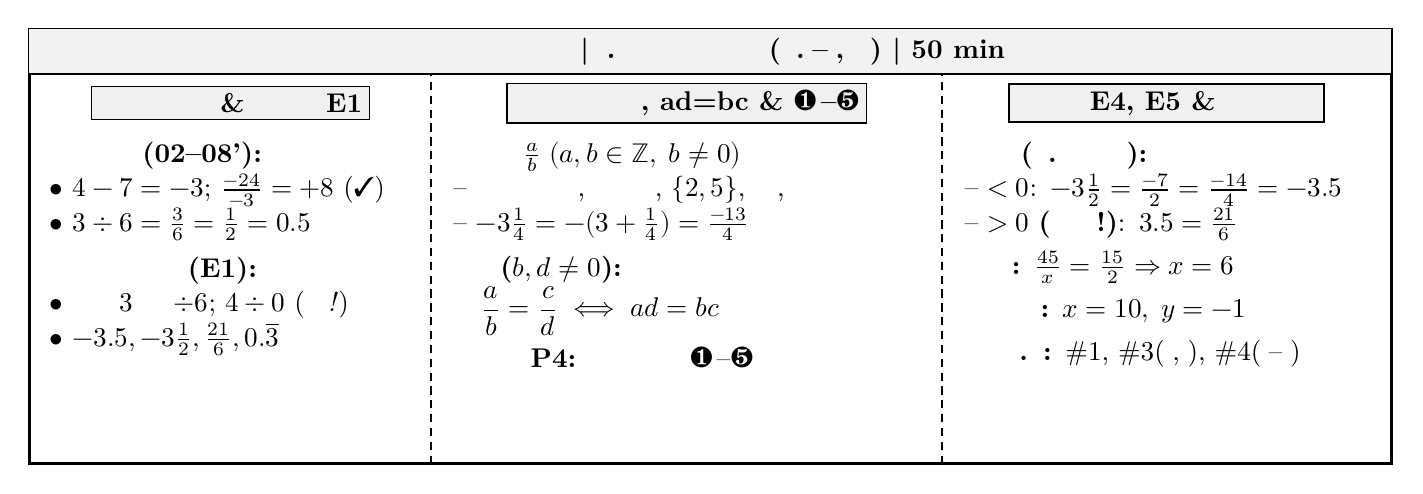
\begin{tikzpicture}[x=0.92cm, y=0.92cm, every node/.style={font=\linespread{1.0}\fontsize{9.8pt}{12.5pt}\selectfont, text=black}]
  \draw[black, line width=1.1pt] (0,0) rectangle (18.80, 6.00);
  \fill[headgray] (0, 5.38) rectangle (18.80, 6.00);
  \draw[black, line width=0.85pt] (0, 5.38) -- (18.80, 5.38);
  \node at (9.40, 5.69) {\textbf{មេរៀនទី១ ចំនួនសនិទាន \en{|} ១. សញ្ញាណចំនួនសនិទាន (ទំ.១–២, ១១) \en{|} \en{50 min}}};

  \draw[black, densely dashed, line width=0.8pt] (5.55, 0) -- (5.55, 5.38);
  \draw[black, densely dashed, line width=0.8pt] (12.60, 0) -- (12.60, 5.38);

  \node[fill=panelgray, draw=black, line width=0.5pt, inner sep=2.5pt] at (2.775, 4.98) {\textbf{តំបន់ ១៖ រំលឹក \& បេសកកម្ម \en{E1}}};
  \node[anchor=north west, align=left, text width=4.90cm] at (0.15, 4.58) {%
    \textbf{មូលដ្ឋានទី៧ (\en{02–08'}):}\\
    $\bullet\ 4-7 = -3$; $\frac{-24}{-3} = +8$ (\ding{51})\\
    $\bullet\ 3\div 6 = \frac{3}{6} = \frac{1}{2} = 0.5$\\[4pt]
    \textbf{ទីផ្សារកំពង់ស្វាយ (\en{E1}):}\\
    $\bullet$ ស្រូវ $3$ បាវ $\div 6$; $4\div 0$ (\textit{ហាម!})\\
    $\bullet$ $-3.5,-3\frac{1}{2},\frac{21}{6},0.\overline{3}$};

  \node[fill=panelgray, draw=black, line width=0.5pt, inner sep=2.5pt] at (9.075, 4.98) {\textbf{តំបន់ ២៖ និយមន័យ, \en{ad=bc} \& \cnum{1}–\cnum{5}}};
  \node[anchor=north west, align=left, text width=6.10cm] at (5.72, 4.58) {%
    \textbf{និយមន័យ៖} $\frac{a}{b}\;(a,b\in\mathbb{Z},\; b\neq 0)$\\
    – ៥ ទម្រង់៖ គត់, រ៉ឺឡាទីប, $\{2,5\}$, ខួប, ចំរុះ\\
    – $-3\frac{1}{4} = -(3+\frac{1}{4}) = \frac{-13}{4}$\\[4pt]
    \textbf{វិធាន ($b,d\neq 0$):}\\
    \quad $\dfrac{a}{b}=\dfrac{c}{d} \iff ad=bc$\\[3pt]
    \textbf{បិទផ្ទាំង \en{P4}:} ធនាគារហេតុផល \cnum{1}–\cnum{5}};

  \node[fill=panelgray, draw=black, line width=0.5pt, inner sep=2.5pt] at (15.70, 4.98) {\textbf{តំបន់ ៣៖ \en{E4}, \en{E5} \& កិច្ចការផ្ទះ}};
  \node[anchor=north west, align=left, text width=5.35cm] at (12.78, 4.58) {%
    \textbf{គំរូ ១ (ទំ.២ កែបំពេញ):}\\
    – $<0$: $-3\frac{1}{2}=\frac{-7}{2}=\frac{-14}{4}=-3.5$\\
    – $>0$ \textbf{(កែខ្វះ!)}: $3.5 = \frac{21}{6}$\\[3pt]
    \textbf{គំរូ ២:} $\frac{45}{x}=\frac{15}{2} \Rightarrow x=6$\\[3pt]
    \textbf{ប្រតិបត្តិ:} $x=10,\; y=-1$\\[3pt]
    \textbf{ផ្ទះ ទំ.១១:} \en{\#1, \#3}(ក,គ), \en{\#4}(ក\en{–}ង)};
\end{tikzpicture}\par
\end{tcolorbox}

\begingroup
\linespread{1.04}\fontsize{10.5pt}{14.8pt}\selectfont
\renewcommand{\arraystretch}{1.12}
\begin{longtable}{|L{4.80cm}|L{6.10cm}|L{6.10cm}|}
\hline
\rowcolor{headgray}
\multicolumn{1}{|C{4.80cm}|}{\tblhead{បញ្ហាដែលជួបក្នុងថ្នាក់}} &
\multicolumn{1}{C{6.10cm}|}{\tblhead{មូលហេតុតាមភស្តុតាងស្រាវជ្រាវ}} &
\multicolumn{1}{C{6.10cm}|}{\tblhead{វិធានការកែតម្រូវភ្លាមៗរបស់គ្រូ}} \\
\hline
\endfirsthead
\hline
\rowcolor{headgray}
\multicolumn{1}{|C{4.80cm}|}{\tblhead{បញ្ហាដែលជួបក្នុងថ្នាក់}} &
\multicolumn{1}{C{6.10cm}|}{\tblhead{មូលហេតុតាមភស្តុតាងស្រាវជ្រាវ}} &
\multicolumn{1}{C{6.10cm}|}{\tblhead{វិធានការកែតម្រូវភ្លាមៗរបស់គ្រូ}} \\
\hline
\endhead
\hline
\endfoot
\hline
\endlastfoot
១. សិស្សអះអាង $\frac{4}{0}=0$ ឬ $\frac{0}{4}=4$ & លាយឡំក្បួនគុណនិងចែកនឹង $0$ \en{(Karakuş \& Aydın, 2019; Yetim \& Alkan, 2013)}។ & សួរ៖ «$? \times 0 = 4$ ស្មើលេខប៉ុន្មាន?» ឱ្យសិស្សឃើញថាគ្មានលេខ $k$ ណាទាំងអស់ ($\neq 0$)។ \\
\hline
២. សិស្សសរសេរ $-3\frac{1}{4}=\frac{-11}{4}$ & ធ្វើ $(-3\times 4)+1$ បាត់វង់ក្រចក \en{(Susiswo et al., 2021)}។ & បង្ហាញលើបន្ទាត់ \en{P1}: ចេញពី $0$ ទៅឆ្វេង $-3$ រួចដើរបន្ថែមឆ្វេង $\frac{1}{4} \Rightarrow -\left(3+\frac{1}{4}\right)=\frac{-13}{4}$។ \\
\hline
៣. សិស្សស្មាន $\frac{1}{2}$ ខួប ព្រោះបឋមនឹងគ្នា & បកស្រាយប្រយោគទំ.១ ហួសព្រំដែន (\en{Nuance \#1})។ & ឱ្យសាកចែក $1\div 2 = 0.5$ និងបង្រៀនលក្ខខណ្ឌ $\{2,5\}$ ធៀប $3$ ($1/3$) និង $163$ ($\frac{17}{652}$)។ \\
\hline
៤. សិស្សភ្លេចផ្គុំ $3.5=\frac{21}{6}$ ក្នុងគំរូ ១ & ផ្ទៀងតាមចម្លើយបោះពុម្ពសៀវភៅទំ.២ ដែលភ្លេច។ & បង្គាប់គូស \en{[tracing]} ញែកក្រុម $<0$ (៤ ចំនួន) ពី $>0$ ($3.5, \frac{21}{6}$: ២ ចំនួន) មុនសរសេរ។ \\
\hline
\end{longtable}
\endgroup

% ============================================================================
% ផ្នែកទី ៥៖ រូបភាពបច្ចេកទេស និងដ្យាក្រាមវិភាគ (Technical B&W TikZ Diagrams)
% ============================================================================
\secbanner{ផ្នែកទី ៥៖ រូបភាពបច្ចេកទេស និងដ្យាក្រាមវិភាគ \enbf{(B\&W Technical Figures)}}{Section 5: Proportional B\&W Diagrams (>= 10pt Labels) Synced with Classroom Kits}

\subsec{៥\enbf{.}១ វិភាគរូបភាពពិសោធន៍ \enbf{E2–E3} \enbf{(}រូបទី ១–២\enbf{)}}

ដើម្បីឱ្យគ្រូបង្ហាញពីទំនាក់ទំនងបរិមាណពិតមុនចូលទម្រង់និមិត្តសញ្ញា \textbf{រូបទី ១} ភ្ជាប់ជញ្ជាំងបត់ \en{1:1} នឹងពិសោធន៍ \en{Dual POE} ដើម្បីទម្លាយអន្ទាក់ $b=0$ និងកត្តា $\{2,5\}$ ចំណែក \textbf{រូបទី ២} បង្រួបបង្រួមទម្រង់ទាំង ៥ តាមរចនាសម្ព័ន្ធ \en{Hub-and-Spoke} ភ្ជាប់ធនាគារហេតុផល \cnum{1}–\cnum{5} ។

% --- រូបទី ១ (width <= 17.6cm, font >= 10pt, taller strips + clean auto-fit POE boxes) ---
\begin{tcolorbox}[enhanced, sharp corners, colback=white, colframe=black, boxrule=0.8pt, top=5pt, bottom=5pt, left=4pt, right=4pt, before skip=2pt, after skip=6pt]
\centering
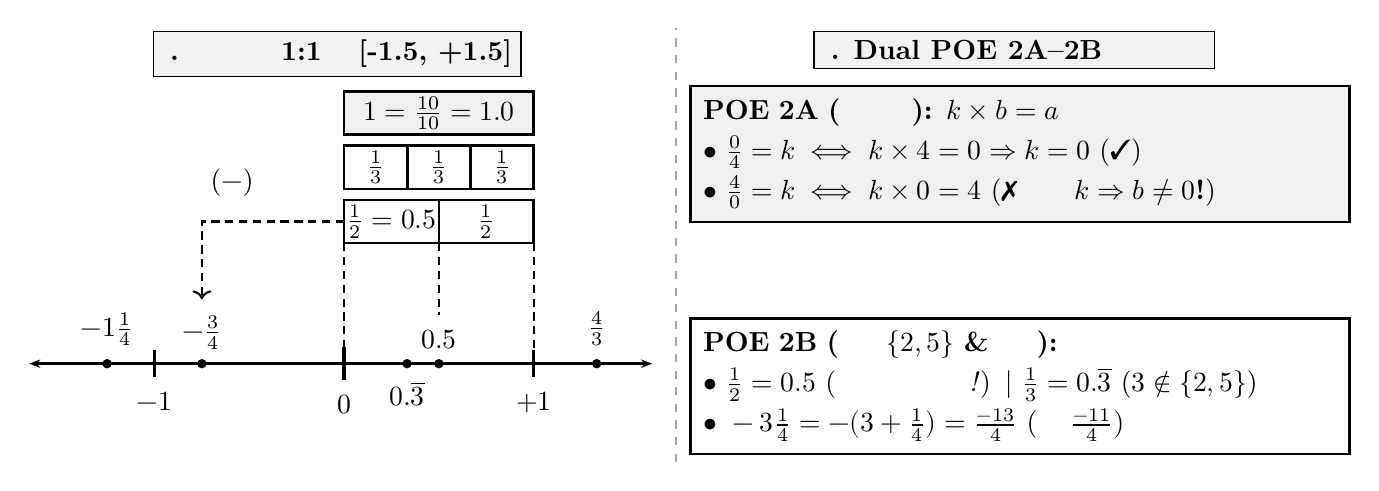
\begin{tikzpicture}[x=0.86cm, y=0.86cm, every node/.style={font=\linespread{1.0}\fontsize{10pt}{13pt}\selectfont, text=black}]
  \draw[line width=0.6pt, dashed, gray!70] (9.80, 0.05) -- (9.80, 6.45);
  \node[anchor=north, fill=headgray, draw=black, line width=0.5pt, inner sep=3.2pt] at (4.80, 6.42) {\textbf{ក. ជញ្ជាំងបត់ \en{1:1} លើ \en{[-1.5, +1.5]}}};
  \node[anchor=north, fill=headgray, draw=black, line width=0.5pt, inner sep=3.2pt] at (14.80, 6.42) {\textbf{ខ. \en{Dual POE 2A–2B} បំបែកអន្ទាក់}};

  % Left: Fraction wall (rows top-down: Whole -> Thirds -> Halves, 1 unit = 2.80 from x=4.90)
  \draw[black, line width=0.95pt, fill=panelgray] (4.90, 4.88) rectangle (7.70, 5.52);
  \node at (6.30, 5.20) {$1 = \frac{10}{10} = 1.0$};
  \draw[black, line width=0.95pt] (4.90, 4.08) rectangle (5.833, 4.72);
  \draw[black, line width=0.95pt] (5.833, 4.08) rectangle (6.767, 4.72);
  \draw[black, line width=0.95pt] (6.767, 4.08) rectangle (7.70, 4.72);
  \node at (5.367, 4.40) {$\frac{1}{3}$};
  \node at (6.300, 4.40) {$\frac{1}{3}$};
  \node at (7.233, 4.40) {$\frac{1}{3}$};
  \draw[black, line width=0.95pt] (4.90, 3.28) rectangle (6.30, 3.92);
  \draw[black, line width=0.95pt] (6.30, 3.28) rectangle (7.70, 3.92);
  \node at (5.60, 3.60) {$\frac{1}{2}=0.5$};
  \node at (7.00, 3.60) {$\frac{1}{2}$};

  % Drop lines stop cleanly above 0.5 label at x=6.30 and arrow stops cleanly above -3/4
  \draw[black, densely dashed, line width=0.7pt] (4.90, 3.28) -- (4.90, 1.50);
  \draw[black, densely dashed, line width=0.7pt] (6.30, 3.28) -- (6.30, 2.22);
  \draw[black, densely dashed, line width=0.7pt] (7.70, 3.28) -- (7.70, 1.50);
  \draw[black, densely dashed, line width=0.75pt, ->] (4.90, 3.60) -- (2.80, 3.60) -- (2.80, 2.45);
  \node[fill=white, inner sep=1.5pt] at (2.55, 4.18) {ត្រឡប់ឆ្វេង ($-$)};

  \draw[{Stealth[length=4pt]}-{Stealth[length=4pt]}, black, line width=1.1pt] (0.25, 1.50) -- (9.45, 1.50);
  \draw[black, line width=1.1pt] (2.10, 1.30) -- (2.10, 1.70); \node[below=2pt] at (2.10, 1.30) {$-1$};
  \draw[black, line width=1.2pt] (4.90, 1.26) -- (4.90, 1.74); \node[below=2pt] at (4.90, 1.26) {$0$};
  \draw[black, line width=1.1pt] (7.70, 1.30) -- (7.70, 1.70); \node[below=2pt] at (7.70, 1.30) {$+1$};
  \fill[black] (1.40, 1.50) circle (1.7pt); \node[above=3pt] at (1.40, 1.50) {$-1\frac{1}{4}$};
  \fill[black] (2.80, 1.50) circle (1.7pt); \node[above=3pt, fill=white, inner sep=1pt] at (2.80, 1.54) {$-\frac{3}{4}$};
  \fill[black] (5.83, 1.50) circle (1.7pt); \node[below=3pt] at (5.83, 1.50) {$0.\overline{3}$};
  \fill[black] (6.30, 1.50) circle (1.7pt); \node[above=3pt, fill=white, inner sep=1pt] at (6.30, 1.54) {$0.5$};
  \fill[black] (8.63, 1.50) circle (1.7pt); \node[above=3pt] at (8.63, 1.50) {$\frac{4}{3}$};

  % Right: Dual POE 2A-2B auto-fitted node boxes (zero border clipping!)
  \node[anchor=north west, draw=black, line width=0.85pt, fill=panelgray, inner sep=4.5pt, align=left, text width=8.05cm] at (10.00, 5.62) {%
    \textbf{POE 2A (អន្ទាក់ ០):} $k\times b = a$\\[1.5pt]
    $\bullet\ \frac{0}{4}=k \iff k\times 4=0 \Rightarrow k=0$ (\ding{51})\\[1.5pt]
    $\bullet\ \frac{4}{0}=k \iff k\times 0=4$ (\ding{55} \textbf{គ្មាន $k \Rightarrow b\neq 0$!})};
  \node[anchor=south west, draw=black, line width=0.85pt, fill=white, inner sep=4.5pt, align=left, text width=8.05cm] at (10.00, 0.15) {%
    \textbf{POE 2B (កត្តា $\{2,5\}$ \& សញ្ញា):}\\[1.5pt]
    $\bullet\ \frac{1}{2}=0.5$ (\textit{បឋមនឹងគ្នា តែដាច់!}) \textbar\ $\frac{1}{3}=0.\overline{3}$ ($3\notin \{2,5\}$)\\[1.5pt]
    $\bullet\ -3\frac{1}{4}=-(3+\frac{1}{4})=\frac{-13}{4}$ (\textbf{ហាម} $\frac{-11}{4}$)};
\end{tikzpicture}\par
\vspace{3pt}
{\fontsize{10.5pt}{14pt}\selectfont\textbf{រូបទី ១៖} ការបត់បន្ទះ \en{1:1} លើបន្ទាត់ចំនួនភ្លោះ និងពិសោធន៍ \en{Dual POE 2A–2B} \en{(Pearn, 2007; Karakuş \& Aydın, 2019; Susiswo et al., 2021; Siegler et al., 2011)}។}
\end{tcolorbox}

\textbf{ចំណុចសង្កេតបច្ចេកទេសពីរូបទី ១៖} នៅពេលដាក់បន្ទះបត់ \en{1:1} លើបន្ទាត់ចំនួនភ្លោះ $[-1.5,+1.5]$ គ្រូគួរចង្អុលឱ្យសិស្សឃើញថា បន្ទាត់ដាច់ៗបង្ហាញការតម្រឹមទីតាំងតែមួយ ($0.5=\frac{1}{2}$) មុននឹងឆ្លុះចម្ងាយដដែលទៅឆ្វេងលេខ $0$ សម្រាប់ $-\frac{3}{4}$ និង $-1\frac{1}{4}$ រួចទើបប្រើសមីការ $k\times b=a$ បញ្ជាក់ភាពគ្មានចម្លើយនៃ $\frac{4}{0}$ ។

% --- រូបទី ២ (E3 Hub-and-Spoke & Warrant Bank ①–⑤) ---
\begin{tcolorbox}[enhanced, sharp corners, colback=white, colframe=black, boxrule=0.8pt, top=5pt, bottom=5pt, left=4pt, right=4pt, before skip=2pt, after skip=6pt]
\centering
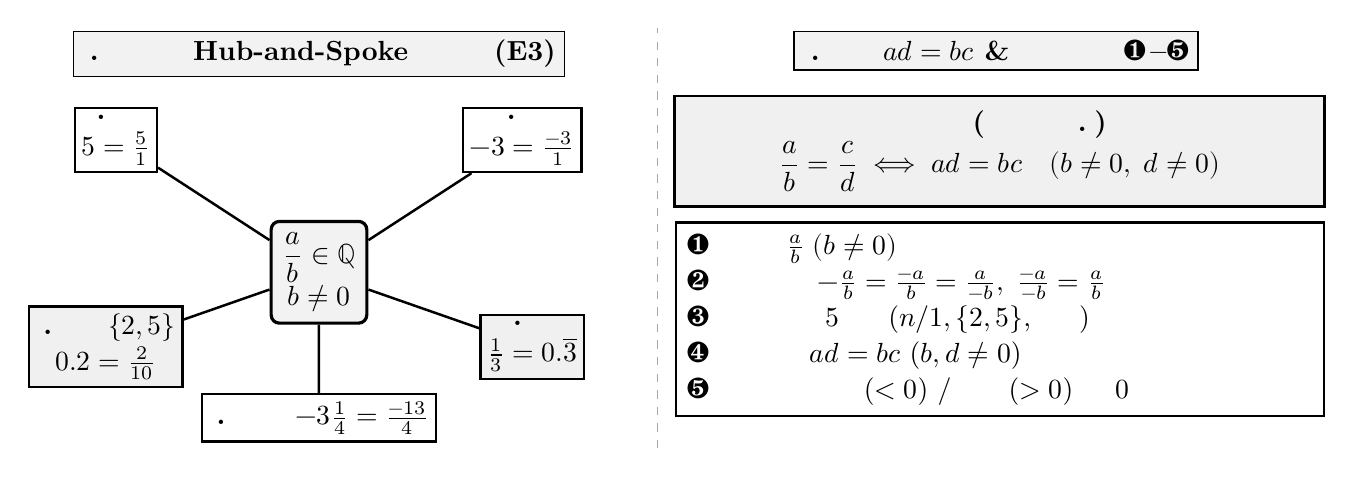
\begin{tikzpicture}[x=0.86cm, y=0.86cm, every node/.style={font=\linespread{1.0}\fontsize{10pt}{13pt}\selectfont, text=black}]
  \draw[line width=0.6pt, dashed, gray!70] (9.80, 0.05) -- (9.80, 6.25);
  \node[anchor=north, fill=headgray, draw=black, line width=0.5pt, inner sep=3.2pt] at (4.80, 6.22) {\textbf{ក. ដ្យាក្រាម \en{Hub-and-Spoke} ៥ ទម្រង់ (\en{E3})}};
  \node[anchor=north, fill=headgray, draw=black, line width=0.5pt, inner sep=3.2pt] at (14.80, 6.22) {\textbf{ខ. វិធាន $ad=bc$ \& ធនាគារហេតុផល \cnum{1}–\cnum{5}}};

  % Left: Hub & 5 Spokes comfortably below header pill
  \node[draw=black, line width=1.15pt, fill=headgray, rounded corners=3pt, inner sep=4pt, align=center] (HUB) at (4.80, 2.65) {$\dfrac{a}{b}\in\mathbb{Q}$\\ $b\neq 0$};
  \node[draw=black, line width=0.8pt, fill=white, inner sep=2.5pt, align=center] (S1) at (1.80, 4.60) {\textbf{១. គត់}\\ $5=\frac{5}{1}$};
  \node[draw=black, line width=0.8pt, fill=white, inner sep=2.5pt, align=center] (S2) at (7.80, 4.60) {\textbf{២. ដក}\\ $-3=\frac{-3}{1}$};
  \node[draw=black, line width=0.8pt, fill=panelgray, inner sep=2.5pt, align=center] (S3) at (1.65, 1.55) {\textbf{៣. ដាច់ $\{2,5\}$}\\ $0.2=\frac{2}{10}$};
  \node[draw=black, line width=0.8pt, fill=panelgray, inner sep=2.5pt, align=center] (S4) at (7.95, 1.55) {\textbf{៤. ខួប}\\ $\frac{1}{3}=0.\overline{3}$};
  \node[draw=black, line width=0.8pt, fill=white, inner sep=2.5pt, align=center] (S5) at (4.80, 0.50) {\textbf{៥. ចំរុះ៖} $-3\frac{1}{4}=\frac{-13}{4}$};
  \draw[black, line width=0.9pt] (HUB) -- (S1) (HUB) -- (S2) (HUB) -- (S3) (HUB) -- (S4) (HUB) -- (S5);

  % Right: ad=bc & Warrant Bank 1-5 clearly below header pill
  \draw[black, line width=0.9pt, fill=panelgray] (10.05, 3.62) rectangle (19.65, 5.25);
  \node[align=center] at (14.85, 4.435) {\textbf{វិធានសមភាព (កែលក្ខខណ្ឌទំ.២)៖}\\ $\dfrac{a}{b}=\dfrac{c}{d} \iff ad=bc \quad (b\neq 0,\; d\neq 0)$};
  \node[anchor=north west, draw=black, fill=white, line width=0.8pt, inner sep=4pt, align=left, text width=7.95cm] at (10.05, 3.40) {%
    \cnum{1} និយមន័យ $\frac{a}{b}\;(b\neq 0)$\\
    \cnum{2} ច្បាប់សញ្ញា $-\frac{a}{b}=\frac{-a}{b}=\frac{a}{-b},\; \frac{-a}{-b}=\frac{a}{b}$\\
    \cnum{3} បម្លែងទម្រង់ $5$ យ៉ាង ($n/1, \{2,5\}$, ចំរុះ)\\
    \cnum{4} ផលគុណខ្វែង $ad=bc$ ($b,d\neq 0$)\\
    \cnum{5} ពិនិត្យសញ្ញាឆ្វេង ($<0$) / ស្ដាំ ($>0$) លេខ $0$};
\end{tikzpicture}\par
\vspace{3pt}
{\fontsize{10.5pt}{14pt}\selectfont\textbf{រូបទី ២៖} រចនាសម្ព័ន្ធ \en{Hub-and-Spoke} បង្រួបបង្រួមទម្រង់ទាំង ៥ និងធនាគារហេតុផល \cnum{1}–\cnum{5} \en{(Xu et al., 2026; Rizos \& Adam, 2022)}។}
\end{tcolorbox}

\subsec{៥\enbf{.}២ វិភាគរូបភាពលំហាត់ \enbf{E4–E5} និងកិច្ចការផ្ទះ \enbf{(}រូបទី ៣–៤\enbf{)}}

\textbf{រូបទី ៣} បង្ហាញការញែកក្រុម \en{[tracing]} ដើម្បីកែបំពេញក្រុមវិជ្ជមាន $3.5=\frac{21}{6}$ នៃគំរូទី ១ និងគម្រោងដំណោះស្រាយគំរូទី ២–ប្រតិបត្តិ ($x=6$; $x=10,y=-1$) រីឯ \textbf{រូបទី ៤} សង្ខេបកាតវិនិច្ឆ័យ \en{A–D} និងគន្លឹះកិច្ចការផ្ទះទំព័រ ១១។

% --- រូបទី ៣ (E4 Model 1 Fixed + Model 2 & E5 Practice) ---
\begin{tcolorbox}[enhanced, sharp corners, colback=white, colframe=black, boxrule=0.8pt, top=5pt, bottom=5pt, left=4pt, right=4pt, before skip=2pt, after skip=6pt]
\centering
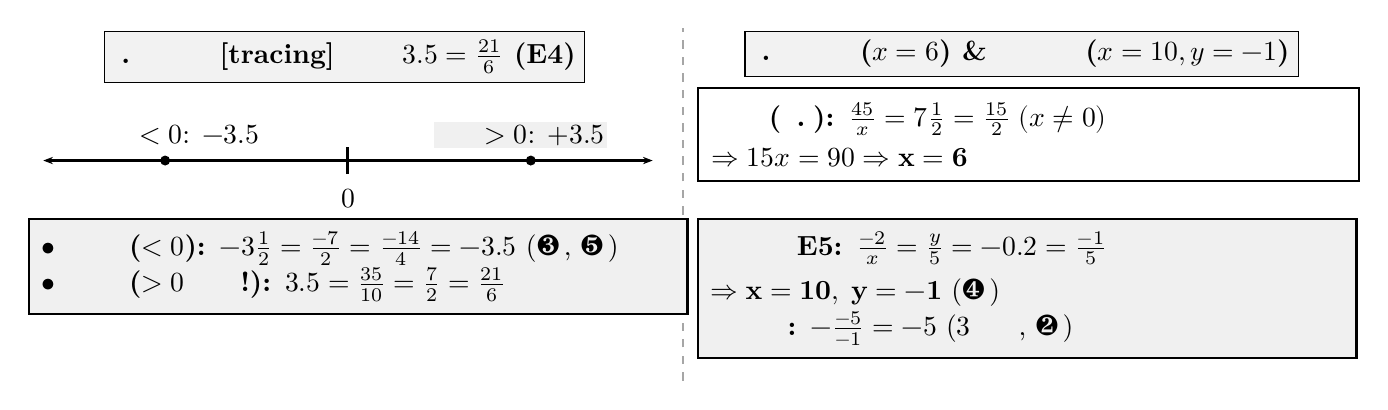
\begin{tikzpicture}[x=0.86cm, y=0.86cm, every node/.style={font=\linespread{1.0}\fontsize{10pt}{13pt}\selectfont, text=black}]
  \draw[line width=0.6pt, dashed, gray!70] (9.80, 0.05) -- (9.80, 5.25);
  \node[anchor=north, fill=headgray, draw=black, line width=0.5pt, inner sep=3.2pt] at (4.80, 5.22) {\textbf{ក. គំរូទី ១ \en{[tracing]} កែខ្វះ $3.5=\frac{21}{6}$ (\en{E4})}};
  \node[anchor=north, fill=headgray, draw=black, line width=0.5pt, inner sep=3.2pt] at (14.80, 5.22) {\textbf{ខ. គំរូទី ២ ($x=6$) \& ប្រតិបត្តិ ($x=10,y=-1$)}};

  % Left: Ex 1 tracing twin groups
  \draw[{Stealth[length=3.5pt]}-{Stealth[length=3.5pt]}, black, line width=1.05pt] (0.35, 3.30) -- (9.35, 3.30);
  \draw[black, line width=1.1pt] (4.85, 3.10) -- (4.85, 3.50);
  \node[below=2pt] at (4.85, 3.10) {$0$};
  \fill[black] (2.15, 3.30) circle (1.8pt);
  \node[above=3pt, fill=white, inner sep=1pt] at (2.30, 3.35) {ក្រុម $<0$: $-3.5$};
  \fill[black] (7.55, 3.30) circle (1.8pt);
  \node[above=3pt, fill=panelgray, inner sep=1pt] at (7.40, 3.35) {ក្រុម $>0$: $+3.5$};

  \node[anchor=north west, draw=black, fill=panelgray, line width=0.75pt, inner sep=4.5pt, align=left, text width=8.05cm] at (0.12, 2.45) {%
    $\bullet$ \textbf{ក្រុម ១ ($<0$):} $-3\frac{1}{2}=\frac{-7}{2}=\frac{-14}{4}=-3.5$ \mbox{(\cnum{3}, \cnum{5})}\\
    $\bullet$ \textbf{ក្រុម ២ ($>0$ កែខ្វះ!):} $3.5 = \frac{35}{10} = \frac{7}{2} = \frac{21}{6}$};

  % Right: Ex 2 & Practice (generous inner padding)
  \node[anchor=north west, draw=black, fill=white, line width=0.75pt, inner sep=5pt, align=left, text width=8.05cm] at (10.00, 4.38) {%
    \textbf{គំរូ ២ (ទំ.២):} $\frac{45}{x}=7\frac{1}{2}=\frac{15}{2}\;(x\neq 0)$\\[1.5pt]
    $\Rightarrow 15x=90 \Rightarrow \mathbf{x=6}$};
  \node[anchor=north west, draw=black, fill=panelgray, line width=0.75pt, inner sep=4.5pt, align=left, text width=8.05cm] at (10.00, 2.45) {%
    \textbf{ប្រតិបត្តិ \en{E5}:} $\frac{-2}{x}=\frac{y}{5}=-0.2=\frac{-1}{5}$\\[3pt]
    $\Rightarrow \mathbf{x=10,\; y=-1}$ \mbox{(\cnum{4})}\\
    \textbf{តេស្តសញ្ញា:} $-\frac{-5}{-1} = -5$ ($3$ ដកសេស, \cnum{2})};
\end{tikzpicture}\par
\vspace{3pt}
{\fontsize{10.5pt}{14pt}\selectfont\textbf{រូបទី ៣៖} កំណែបំពេញ $3.5=\frac{21}{6}$ ក្នុងលំហាត់គំរូទី ១ (\en{E4}) និងគម្រោងដំណោះស្រាយគំរូទី ២–ប្រតិបត្តិ (\en{E5}) \en{(Barbieri et al., 2023; Yeo \& Tzeng, 2019)}។}
\end{tcolorbox}

% --- រូបទី ៤ (E5 Cards A–D & Homework pp. 11 Key) ---
\begin{tcolorbox}[enhanced, sharp corners, colback=white, colframe=black, boxrule=0.8pt, top=5pt, bottom=5pt, left=4pt, right=4pt, before skip=2pt, after skip=6pt]
\centering
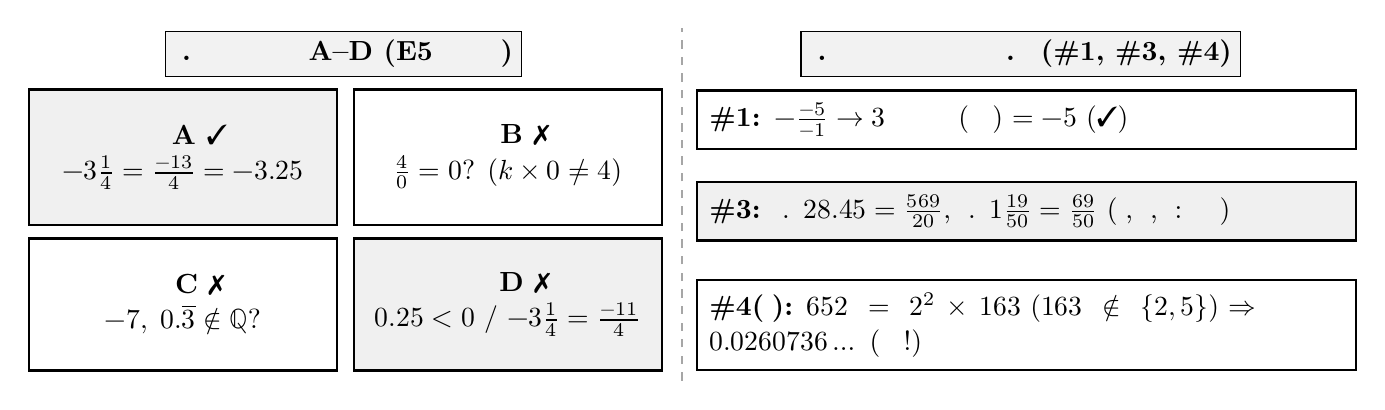
\begin{tikzpicture}[x=0.86cm, y=0.86cm, every node/.style={font=\linespread{1.0}\fontsize{10pt}{12.8pt}\selectfont, text=black}]
  \draw[line width=0.6pt, dashed, gray!70] (9.80, 0.05) -- (9.80, 5.25);
  \node[anchor=north, fill=headgray, draw=black, line width=0.5pt, inner sep=3.2pt] at (4.80, 5.22) {\textbf{ក. កាតវិនិច្ឆ័យ \en{A–D} (\en{E5} ទំព័រ ៥)}};
  \node[anchor=north, fill=headgray, draw=black, line width=0.5pt, inner sep=3.2pt] at (14.80, 5.22) {\textbf{ខ. គន្លឹះកិច្ចការផ្ទះ ទំ.១១ (\en{\#1, \#3, \#4})}};

  % Left 2x2 Cards A-D
  \draw[black, line width=0.8pt, fill=panelgray] (0.15, 2.35) rectangle (4.70, 4.35);
  \node[align=center] at (2.425, 3.35) {\textbf{កាត \en{A} \ding{51}}\\ $-3\frac{1}{4}=\frac{-13}{4}=-3.25$};
  \draw[black, line width=0.8pt] (4.95, 2.35) rectangle (9.50, 4.35);
  \node[align=center] at (7.225, 3.35) {\textbf{កាត \en{B} \ding{55}}\\ $\frac{4}{0}=0$? ($k\times 0\neq 4$)};
  \draw[black, line width=0.8pt] (0.15, 0.20) rectangle (4.70, 2.15);
  \node[align=center] at (2.425, 1.175) {\textbf{កាត \en{C} \ding{55}}\\ $-7,\; 0.\overline{3}\notin\mathbb{Q}$?};
  \draw[black, line width=0.8pt, fill=panelgray] (4.95, 0.20) rectangle (9.50, 2.15);
  \node[align=center] at (7.225, 1.175) {\textbf{កាត \en{D} \ding{55}}\\ $0.25<0$ / $-3\frac{1}{4}=\frac{-11}{4}$};

  % Right HW Hints (#1, #3, #4) wider to keep #3 cleanly on 1 line
  \node[anchor=north west, draw=black, fill=white, line width=0.8pt, inner sep=4.5pt, align=left, text width=8.05cm] at (10.00, 4.35) {%
    \textbf{\#1:} $-\frac{-5}{-1} \to 3$ សញ្ញាដក (សេស) $= -5$ (\ding{51})};
  \node[anchor=north west, draw=black, fill=panelgray, line width=0.8pt, inner sep=4.5pt, align=left, text width=8.05cm] at (10.00, 3.00) {%
    \textbf{\#3:} ក. $28.45=\frac{569}{20}$, គ. $1\frac{19}{50}=\frac{69}{50}$ (ខ, ឃ, ង: ខួប)};
  \node[anchor=north west, draw=black, fill=white, line width=0.8pt, inner sep=4.5pt, align=left, text width=8.05cm] at (10.00, 1.55) {%
    \textbf{\#4(ង):} $652 = 2^2 \times 163$ ($163 \notin \{2,5\}$) $\Rightarrow 0.0260736\dots$ (ខួប!)};
\end{tikzpicture}\par
\vspace{3pt}
{\fontsize{10.5pt}{14pt}\selectfont\textbf{រូបទី ៤៖} កាតវិនិច្ឆ័យ \en{A–D} បង្ការកំហុស \enit{Negz}/សូន្យ និងគន្លឹះកិច្ចការផ្ទះទំ.១១ \en{(McLaren et al., 2012; Žakelj \& Klančar, 2024)}។}
\end{tcolorbox}

\textbf{សំយោគអនុវត្តពីរូបទី ៣–៤៖} គ្រូត្រូវធានាថាក្នុងដំណាក់កាល \en{E4} សិស្សប្រើខ្មៅដៃអូសគំនូស \en{[tracing]} ញែកក្រុម $<0$ ពី $>0$ មុនធ្វើប្រមាណវិធី ដើម្បីរកឃើញគូស្មើគ្នាទី ២ ($3.5=\frac{21}{6}$) ហើយក្នុង \en{E5} ត្រូវឈប់ផ្ដល់ហេតុផលតាមកាត \en{A–D} មុនដាក់សំបុត្រចេញ។

% ============================================================================
% ផ្នែកទី ៦៖ មគ្គុទ្ទេសក៍រៀបចំសម្ភារៈបោះពុម្ព (P1–P6) & ចម្លើយគំរូពេញលេញ
% ============================================================================
\secbanner{ផ្នែកទី ៦៖ មគ្គុទ្ទេសក៍សម្ភារៈបោះពុម្ព \enbf{(Pages 1–6)} និងចម្លើយគំរូពេញលេញ}{Section 6: Printing Calibration (Actual Size 100\%), Classroom Distribution \& Master Answer Keys}

\subsec{៦\enbf{.}១ ស្តង់ដារបោះពុម្ព \enbf{Actual Size 100\%} និងលំដាប់ចែកសន្លឹកកិច្ចការ}

\begin{enumerate}[leftmargin=0.65cm, itemsep=1.5pt]
  \item \textbf{ការកំណត់បោះពុម្ព \en{1:1} ដាច់ខាត (ទំព័រ ១)៖} បោះពុម្ព \en{Printable\_\allowbreak Materials\_\allowbreak RN1.pdf} ដោយជ្រើស \textbf{\en{Scale: Actual Size 100\%}} (\textit{ហាម} \en{Fit to Page}) និងវាស់ផ្ទៀង\textbf{បន្ទះក្រិត \en{5.00 cm}} (\en{141.73 pt}) នៅខាងលើស្ដាំទំព័រ ១ ដើម្បីធានាថាបន្ទះកាត់ \en{A–D} នីមួយៗមានប្រវែង \en{6.00 cm = 1 unit} ពិត និងបន្ទាត់ភ្លោះ $[-1.5, +1.5]$ ប្រវែង $18.00\unit{cm}$ ពិត។
  \item \textbf{សន្លឹកសន្សំក្រដាស \en{B\&W} (ទំព័រ ២–៦)៖} ទំព័រ ២ (កាត \en{E4} គំរូទី ១–២) និងទំព័រ ៣ (សន្លឹក \en{Relay 3} តួនាទី \en{E5}) ជាទម្រង់ \en{2-up}; ទំព័រ ៤ (ផ្ទាំង \en{Hub-and-Spoke} \& \cnum{1}–\cnum{5}) គួរបោះលើក្រដាសរឹង \en{180 gsm} បិទក្ដារខៀន; ទំព័រ ៥ ជាកាត \en{A–D} \en{4-up} + ចម្លើយគ្រូ + សំបុត្រចេញ \en{2-up}; ទំព័រ ៦ ជាប័ណ្ណកិច្ចការផ្ទះ \en{4-up}។
  \item \textbf{ឧបករណ៍តុក្រុម ៣ នាក់ និងពេលចែក៖} កន្ត្រៃ ១, បន្ទាត់ \en{cm} ១, ខ្មៅដៃ \en{[tracing]} ។ ចែកទំព័រ ១ ផ្កាប់នៅនាទី ០០', ទំព័រ ២ នៅនាទី ២៨', ទំព័រ ៣ នៅនាទី ៣៨', បង្ហាញទំព័រ ៥ នៅនាទី ៤៣', និងចែកទំព័រ ៦ នៅនាទី ៤៨'។
\end{enumerate}

\Needspace{4.2cm}
\subsec{៦\enbf{.}២ ចម្លើយគំរូពេញលេញសម្រាប់គ្រប់សន្លឹកកិច្ចការ និងលំហាត់ \enbf{(Master Key)}}

\begingroup
\linespread{1.06}\fontsize{10.2pt}{14.8pt}\selectfont
\renewcommand{\arraystretch}{1.22}
\begin{longtable}{|L{3.05cm}|L{14.20cm}|}
\hline
\rowcolor{headgray}
\multicolumn{1}{|C{3.05cm}|}{\tblhead{សន្លឹក \enbf{/} លំហាត់}} &
\multicolumn{1}{C{14.20cm}|}{\tblhead{ចម្លើយគំរូផ្លូវការ និងពិន្ទុត្រួតពិនិត្យ \enbf{(Master Key)}}} \\
\hline
\endfirsthead
\hline
\rowcolor{headgray}
\multicolumn{1}{|C{3.05cm}|}{\tblhead{សន្លឹក \enbf{/} លំហាត់}} &
\multicolumn{1}{C{14.20cm}|}{\tblhead{ចម្លើយគំរូផ្លូវការ និងពិន្ទុត្រួតពិនិត្យ \enbf{(Master Key)}}} \\
\hline
\endhead
\hline
\endfoot
\hline
\endlastfoot
\textbf{ទំព័រ ១ (\en{E2})}\newline បត់ \en{1:1} & \textbf{បន្ទះ \en{A–D} លើ $[-1.5,+1.5]$:} $\frac{1}{2}=\frac{5}{10}=\frac{3}{6}=0.5$; $\frac{1}{3}=0.\overline{3}$; $\frac{4}{3}=1\frac{1}{3}=1.\overline{3}$; ឆ្លុះឆ្វេង $0$ បាន $-\frac{3}{4}=-0.75$ និង $-1\frac{1}{4}=\frac{-5}{4}$។ \\
\hline
\textbf{ទំព័រ ១ (\en{E2})}\newline \en{Dual POE 2A–2B} & \textbf{\en{POE 2A}:} $\frac{0}{4}=0$ ($0\times 4=0$); $\frac{4}{0}$ គ្មានន័យ (គ្មាន $k\times 0=4 \Rightarrow \mathbf{b\neq 0}$); $\frac{0}{0}$ មិនកំណត់។ \textbf{\en{POE 2B}:} $\frac{1}{2}=\mathbf{0.5}$ (បឋមនឹងគ្នា តែដាច់ ព្រោះកត្តា $\{2,5\}$) vs $\frac{1}{3}=0.\overline{3}$; $-3\frac{1}{4}=-(3+\frac{1}{4})=\mathbf{\frac{-13}{4}}$ \mbox{(ហាម $\frac{-11}{4}$)}; $ad=\mathbf{bc}$។ \\
\hline
\textbf{ទំព័រ ២ (\en{E4})}\newline គំរូ ១ \& ២ (ទំ.២) & \textbf{គំរូ ១:} $<0$: $-3\frac{1}{2}=\frac{-7}{2}=\frac{-14}{4}=-3.5$ (\cnum{3}, \cnum{5}); $>0$ \textbf{(បំពេញសៀវភៅខ្វះ!)}: $3.5=\frac{35}{10}=\frac{7}{2}=\mathbf{\frac{21}{6}}$។ \textbf{គំរូ ២:} $\frac{45}{x}=7\frac{1}{2}=\frac{15}{2}\;(x\neq 0) \Rightarrow 15x=90 \Rightarrow \mathbf{x=6}$ (\cnum{1}, \cnum{4})។ \textbf{\en{EIA}:} $-3\frac{1}{2}=-(3+\frac{1}{2})=\frac{-7}{2}\neq\frac{-5}{2}$ និងមិនត្រូវទុកក្រុម $3.5=\frac{21}{6}$ ចោលឡើយ! \\
\hline
\textbf{ទំព័រ ៣ (\en{E5})}\newline \en{Relay 3} តួនាទី & \textbf{ប្រតិបត្តិ (ទំ.២):} $-0.2=\frac{-2}{10}=\frac{-1}{5}$ (\cnum{3}), $x>0$ និង $x\neq 0$; $\frac{-2}{x}=\frac{-1}{5}\Rightarrow \mathbf{x=10}$; $\frac{y}{5}=\frac{-1}{5}\Rightarrow \mathbf{y=-1}$ (\cnum{4})។ \textbf{តេស្តសញ្ញា:} $-\frac{-5}{-1}$ មាន $3$ ដក (សេស) $= \mathbf{-5}$ (\cnum{2})។ \textbf{បិទ \en{E1}:} $3\div 6,-3,0.5,0.\overline{3}\in\mathbb{Q}$ តែ $4\div 0$ ហាម ($b\neq 0$)។ \\
\hline
\textbf{ទំព័រ ៥ (\en{E5})}\newline កាត \en{A–D} \& សំបុត្រចេញ & \textbf{កាត \en{A–D}:} \textbf{A} \ding{51} ($-3\frac{1}{4}=\frac{-13}{4}=-3.25$); \textbf{B} \ding{55} ($\frac{4}{0}$ គ្មានន័យ); \textbf{C} \ding{55} ($-7=\frac{-7}{1}, 0.\overline{3}=\frac{1}{3}\in\mathbb{Q}$); \textbf{D} \ding{55} ($0.25>0$ មិនមែន $<0$ និង $-3\frac{1}{4}=\frac{-13}{4}$)! \textbf{សំបុត្រចេញ:} ១) $-2\frac{3}{4}=\mathbf{\frac{-11}{4}=-2.75}$; ២) $\frac{0}{-5}=\mathbf{0\in\mathbb{Q}}$ តែ $\frac{-5}{0}$ គ្មានន័យ; ៣) $\frac{12}{m}=\frac{-3}{5}\Rightarrow \mathbf{m=-20}$។ \\
\hline
\textbf{ទំព័រ ៦ (ផ្ទះ)}\newline ទំ.១១ \en{\#1, \#3, \#4} & \textbf{\#1:} ស្មើ $-5$ គឺ $\mathbf{\frac{-5}{1},\; \frac{5}{-1},\; -\frac{5}{1},\; -\frac{-5}{-1}}$ (សេស: ១ ឬ ៣ ដក)។ \textbf{\#3:} \textbf{ក.} $28.45=\frac{2845}{100}=\mathbf{\frac{569}{20}}$; \textbf{គ.} $1\frac{19}{50}=\mathbf{\frac{69}{50}}$ (\textit{ខ, ឃ, ង ជាទសភាគខួប})។ \textbf{\#4:} \textbf{ក.} $0.07$; \textbf{ខ.} $0.0013$; \textbf{គ.} $0.1875$; \textbf{ឃ.} $0.175$; \textbf{ង.} $\frac{17}{652}\approx \mathbf{0.0260736\dots}$ (ទសភាគខួប ៨១ ខ្ទង់ ព្រោះ $652=2^2\times 163$)។ \\
\hline
\end{longtable}
\endgroup

% ============================================================================
% ផ្នែកទី ៧៖ បញ្ជីឯកសារយោង (References --- APA 7th Edition) & ហត្ថលេខា
% ============================================================================
\secbanner{ផ្នែកទី ៧៖ បញ្ជីឯកសារយោង \enbf{(References — APA 7th Edition)}}{Section 7: Verified Open-Access Reference List (100\% 1-to-1 Match with 00\_Evidence\_Index.md \& PDFs 01–15)}

{\TimesEn\linespread{1.0}\selectfont\fontsize{10.8pt}{17.4pt}\selectfont
\setlength{\parskip}{6.0pt}
\everypar={\hangindent=0.85cm \hangafter=1}

Barbieri, C. A., Booth, J. L., \& Chawla, K. (2023). Let’s be rational: Worked examples supplemented textbooks improve conceptual and fraction knowledge. \textit{Educational Psychology}, \textit{43}(1), 1–21. \url{https://doi.org/10.1080/01443410.2022.2144142}

Di Lonardo Burr, S. M., Xu, C., Li, H., Si, J., Huang, B., \& Guo, K. (2026). Finding their way: Students’ fraction misconceptions and errors over two years of fraction learning. \textit{Learning and Instruction}, \textit{106}, Article 102454. \url{https://doi.org/10.1016/j.learninstruc.2026.102454}

Gorman, A., Way, J., \& Bobis, J. (2025). Changing structures of attention when learning about decimal fractions with digital tools. \textit{Education Sciences}, \textit{15}(11), Article 1453. \url{https://doi.org/10.3390/educsci15111453}

Heemsoth, T., \& Heinze, A. (2013). Learning fractions from errors. In A. M. Lindmeier \& A. Heinze (Eds.), \textit{Proceedings of the 37th Conference of the International Group for the Psychology of Mathematics Education} (Vol. 3, pp. 25–32). PME.

Karakuş, F., \& Aydın, B. (2019). Elementary mathematics teachers’ specialized content knowledge related to division by zero. \textit{Malaysian Online Journal of Educational Sciences}, \textit{7}(2), 25–40. (ERIC Document No. EJ1213990). \url{https://files.eric.ed.gov/fulltext/EJ1213990.pdf}

Lemonidis, C., \& Pilianidis, N. (2020). The 8th grade students’ competencies in alternating different symbolic representations of rational numbers. \textit{International Electronic Journal of Mathematics Education}, \textit{15}(3), Article em0587. \url{https://doi.org/10.29333/iejme/7865}

McLaren, B. M., Adams, D., Durkin, K., Goguadze, G., Mayer, R. E., Rittle-Johnson, B., Sosnovsky, S., Isotani, S., \& Van Velsen, M. (2012). To err is human, to explain and correct is divine: A study of interactive erroneous examples with middle school math students. In A. Ravenscroft, S. Lindstaedt, C. Delgado Kloos, \& D. Hernández-Leo (Eds.), \textit{Proceedings of EC-TEL 2012: Seventh European Conference on Technology Enhanced Learning} (LNCS Vol. 7563, pp. 222–235). Springer. \url{https://doi.org/10.1007/978-3-642-33263-0_18}

Pearn, C. A. (2007). Using paper folding, fraction walls, and number lines to develop understanding of fractions for students from Years 5–8. \textit{Australian Mathematics Teacher}, \textit{63}(4), 31–36. (ERIC Document No. EJ779071). \url{https://files.eric.ed.gov/fulltext/EJ779071.pdf}

Rizos, I., \& Adam, M. (2022). Mathematics students’ conceptions and reactions to questions concerning the nature of rational and irrational numbers. \textit{International Electronic Journal of Mathematics Education}, \textit{17}(3), Article em0686. \url{https://doi.org/10.29333/iejme/11977}

Siegler, R. S., Thompson, C. A., \& Schneider, M. (2011). An integrated theory of whole number and fractions development. \textit{Cognitive Psychology}, \textit{62}(4), 273–296. \url{https://doi.org/10.1016/j.cogpsych.2011.03.001}

Susiswo, Murniasih, T. R., Sa’dijah, C., Muksar, M., \& Murtafiah, W. (2021). The development of an instrument on negative fractions to measure the cognitive obstacle based on mental mechanism stages. \textit{TEM Journal}, \textit{10}(3), 1357–1362. \url{https://doi.org/10.18421/TEM103-44}

Xu, Z., Zou, Y., Jin, C., \& Li, L. (2026). Help students construct a hub-and-spoke cognitive structure: A key pathway to reduce burden and improve quality in mathematics classroom teaching. \textit{Frontiers in Psychology}, \textit{17}, Article 1974303. \url{https://doi.org/10.3389/fpsyg.2026.1974303}

Yeo, L.-M., \& Tzeng, Y.-T. (2019). Tracing effect in the worked examples-based learning: An exploration of individual differences in working memory capacity. \textit{Eurasia Journal of Mathematics, Science and Technology Education}, \textit{15}(10), Article em1760. \url{https://doi.org/10.29333/ejmste/105482}

Yetim, S., \& Alkan, R. (2013). How middle school students deal with rational numbers? A mixed methods research study. \textit{Eurasia Journal of Mathematics, Science and Technology Education}, \textit{9}(2), 213–221. \url{https://doi.org/10.12973/eurasia.2013.9211a}

Žakelj, A., \& Klančar, A. (2024). Examining the conceptual and procedural knowledge of decimal numbers in sixth-grade elementary school students. \textit{European Journal of Educational Research}, \textit{13}(3), 1227–1245. \url{https://doi.org/10.12973/eu-jer.13.3.1227}
\par}

\vspace{14pt}
\Needspace{2.2cm}
\hfill
\begin{minipage}{9.8cm}
  {\centering
    ថ្ងៃចន្ទ ៨រោច ខែអស្សុជ ឆ្នាំមមី អដ្ឋស័ក ពុទ្ធសករាជ ២៥៧០\\[2pt]
    កំពង់ស្វាយ, ថ្ងៃទី២ ខែវិច្ឆិកា ឆ្នាំ២០២៦\\[3pt]
    {\muol គ្រូបង្រៀន}\par}
  \vspace{32pt}
  \hfill{\muol ហុក ប៊ុនថែន}\hspace*{1.4cm}
\end{minipage}

\end{document}
